\documentclass{beamer}
\usepackage{amsmath,amsfonts,amsthm,amssymb,chemformula,graphicx,multicol,multirow,tikz,xcolor}
\usepackage[backend=biber,sorting=none,style=numeric-comp,giveninits]{biblatex}
\usetikzlibrary{matrix, fit}

\DeclareNameAlias{default}{family-given}
\renewbibmacro{in:}{}
\addbibresource{references.bib}

\usetheme{Madrid}
\usefonttheme{professionalfonts}

\newcommand{\vs}{\vspace{5mm}}

\DeclareMathOperator{\Gal}{Gal}
\DeclareMathOperator{\tr}{tr}

\newtheorem{proposition}{Proposition}
\setbeamertemplate{theorems}[numbered]

\setbeamertemplate{page number in head/foot}{}

\title[Molecular Symmetry Point Groups]{Cyclotomic Structure and Galois Actions\\of Molecular Symmetry Point Groups}
\author[Margaret A. Barker]{\texorpdfstring{Margaret A. Barker\\Advisor: Dr. Lilit Martirosyan}{Margaret A. Barker, Advisor: Dr. Lilit Martirosyan}}
\institute[UNCW]{University of North Carolina Wilmington\\Department of Mathematics and Statistics}
\date[April 27, 2026]{April 27, 2026}

\begin{document}
    \frame{\titlepage}
    
    \begin{frame}{Table of contents}
        \tableofcontents[sections=1-8]
    \end{frame}

    \section{Introduction}

    \begin{frame}{Introduction}
    Symmetry connects the world we see with chemistry, and the language of symmetry is algebra. Countless chemical processes are connected to molecular symmetry, and a deep understanding of these concepts is rooted in group theory, representation theory, and character theory.
    \vs

    \onslide<2->
    {
        In this project, we will do the following:
        \begin{enumerate}
            \item Introduce notation of molecular point groups and discuss how to categorize molecules by point group.
            \item Derive character tables from matrix representations, focusing in particular on $C_{2v}$ and $C_{3v}$, the point groups of water (\ch{H2O}) and ammonia (\ch{NH3}), respectively.
            \item Decompose the matrix representations into irreducible representations using properties of character tables.
            \item Analyze the character table entries from the point of view of linear algebra and number theory.
        \end{enumerate}
    }
    \end{frame}

    \begin{frame}{Introduction}
        We will show that, in general, eigenvalues of symmetry operations lie in cyclotomic fields, and that their minimal polynomials factor into cyclotomic polynomials.
        \vs
    
        \onslide<2->
        {
            We will see that these eigenvalues are roots of unity, and characters lie in cyclotomic fields such as $\mathbb{Q}(\zeta_n)$.
        }
        \vs
    
        \onslide<3->
        {
            This analysis leaves some questions unanswered, such as why the characters of $C_{3v}$ are all integers, despite lying in the cyclotomic field $\mathbb{Q}(\zeta_3)$.
        }
        \vs
    
        \onslide<4->
        {
            To gain a deeper understanding, we will pivot to Galois theory. We look at the behavior of primitive $n$th roots of unity and eigenvalues under Galois automorphisms, which will help explain why the characters of $C_{3v}$ lie in $\mathbb{Z}$.
        }
    \end{frame}

    \begin{frame}{Introduction}
        However, some character tables do not have integer characters. In particular, some molecules with fivefold symmetries belong to point groups whose character values involve the golden ratio, and we will see that under the same Galois automorphisms, the relevant Galois-invariant character values lie in $\mathbb{Q}(\sqrt{5})$ rather than in $\mathbb{Q}(\zeta_5)$ or $\mathbb{Q}$.
        \vs

        \onslide<2->
        {
            The central idea of this project is that the eigenvalues of symmetry operations lie in cyclotomic fields, and the action of the corresponding Galois groups explains the algebraic structure of the character values appearing in molecular point group representations.
        }
        \vs

        \onslide<3->
        {
            Much of the presentation of point groups and character theory, up until the discussion of minimal polynomials and eigenvalues, follows the treatments in \cite{miessler2014,mcgrady2024,vallance,young}.
        }
    \end{frame}

    \section{Molecular point groups}

    \begin{frame}{Molecular point groups}
        Many molecules contain \emph{symmetry elements} upon which \emph{symmetry operations} can be performed. A molecule is indistinguishable before and after any symmetry operation it possesses.
        \vs
    
        \onslide<2->
        {
            The identity operation, $E$, does nothing. It is required in order to express a collection of symmetries as a group.
        }
        \vs

        \onslide<3->
        {
            Let $n\geq2$ be an integer. A proper rotation, $C_n$, is a rotation through $360^\circ/n$ with respect to some axis. We have that $C_n^n\equiv E$, so $|C_n|=n$.
        }
        \vs

        \onslide<4->
        {
            If a molecule has more than one rotational axis, the one of highest order is called the \emph{principal axis}.
        }
    \end{frame}

    \begin{frame}{Molecular point groups}\small
        A mirror-plane reflection is denoted $\sigma$. If it is perpendicular to the principal axis, it is called horizontal and denoted $\sigma_h$. If it includes the principal axis, it is called vertical and denoted $\sigma_v$. A vertical reflection plane that bisects the angle between two $C_2$ axes is called dihedral and denoted $\sigma_d$.
        \vs

        \onslide<2->
        {
            The inversion operation, $i$, is where every point of the molecule is reflected with respect to the center of the molecule.
        }
        \vs

        \onslide<3->
        {
            An improper rotation, $S_n$, also called a rotation-reflection, is a $C_n$ rotation followed by a $\sigma_h$ reflection through a plane perpendicular to the rotation axis.
        }
        \vs

        \onslide<4->
        {
            The collection of symmetry operations that a molecule possesses determines its \emph{point group}. At least one point in space is invariant under each symmetry operation, and the symmetry elements and operations have a group structure. We use Schoenflies notation to denote point groups, following standard conventions in chemistry.
        }
    \end{frame}

    \begin{frame}{Categorization of molecules into point groups}
        We follow a sequence of steps to determine the point group of a molecule.
        \vs
        
        To get started, we can classify molecules as being of \emph{low symmetry}, \emph{high symmetry}, or neither. We will list the point groups of the three categories and show example molecules that exhibit each group.
        \vs
        
        To assist in determining the point groups for molecules of neither low nor high symmetry, we will use a flowchart.
    \end{frame}

    \begin{frame}{Point groups of low symmetry}
        Molecules in the $C_1$ group have no symmetry besides the identity. (Indeed, every point group has the identity, but it will not be mentioned in the following groups.) An example is bromochlorofluoromethane (\ch{CHBrClF}).

        \begin{center}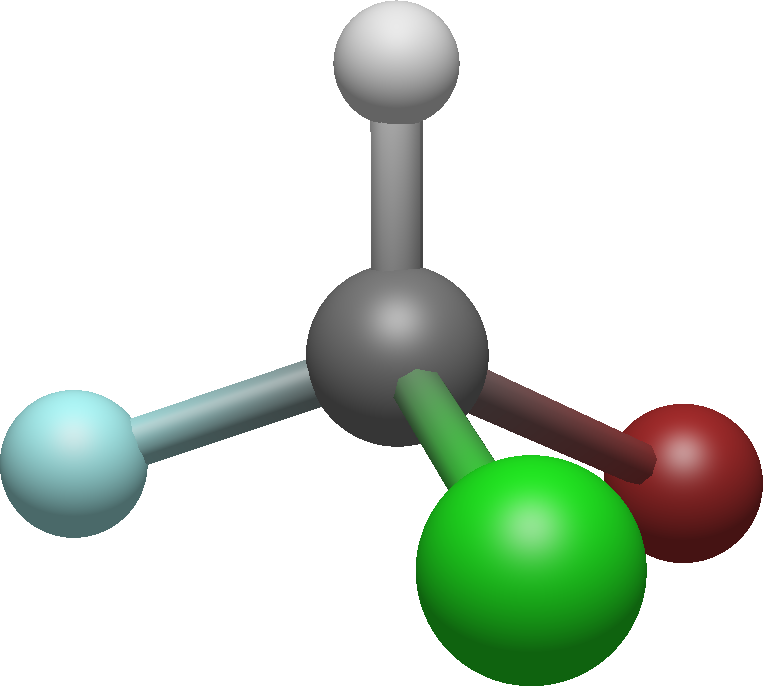
\includegraphics[width=1in]{figures/c1example.png}\end{center}
        
        \onslide<2->
        {
            Molecules in the $C_s$ group have only one mirror plane (in the following example, the mirror plane is the plane of the molecule). An example is 1-bromo-1-chloroethene (\ch{C2H2BrCl}).
    
            \begin{center}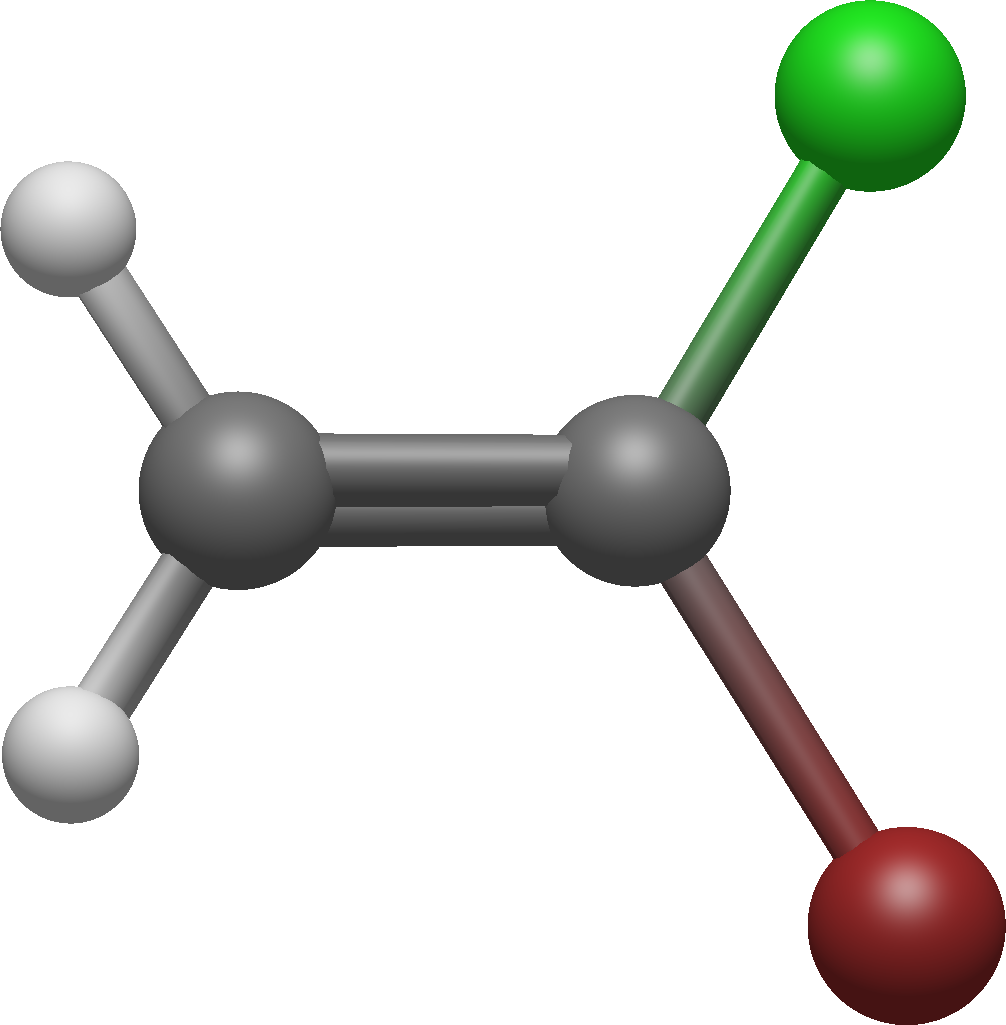
\includegraphics[width=0.75in]{figures/csexample.png}\end{center}
        }
    \end{frame}

    \begin{frame}{Point groups of low symmetry}
        Molecules in the $C_i$ group have only an inversion center. An example is 1,2-dibromo-1,2-dichloroethane (\ch{C2H2Br2Cl2}).
    
        \begin{center}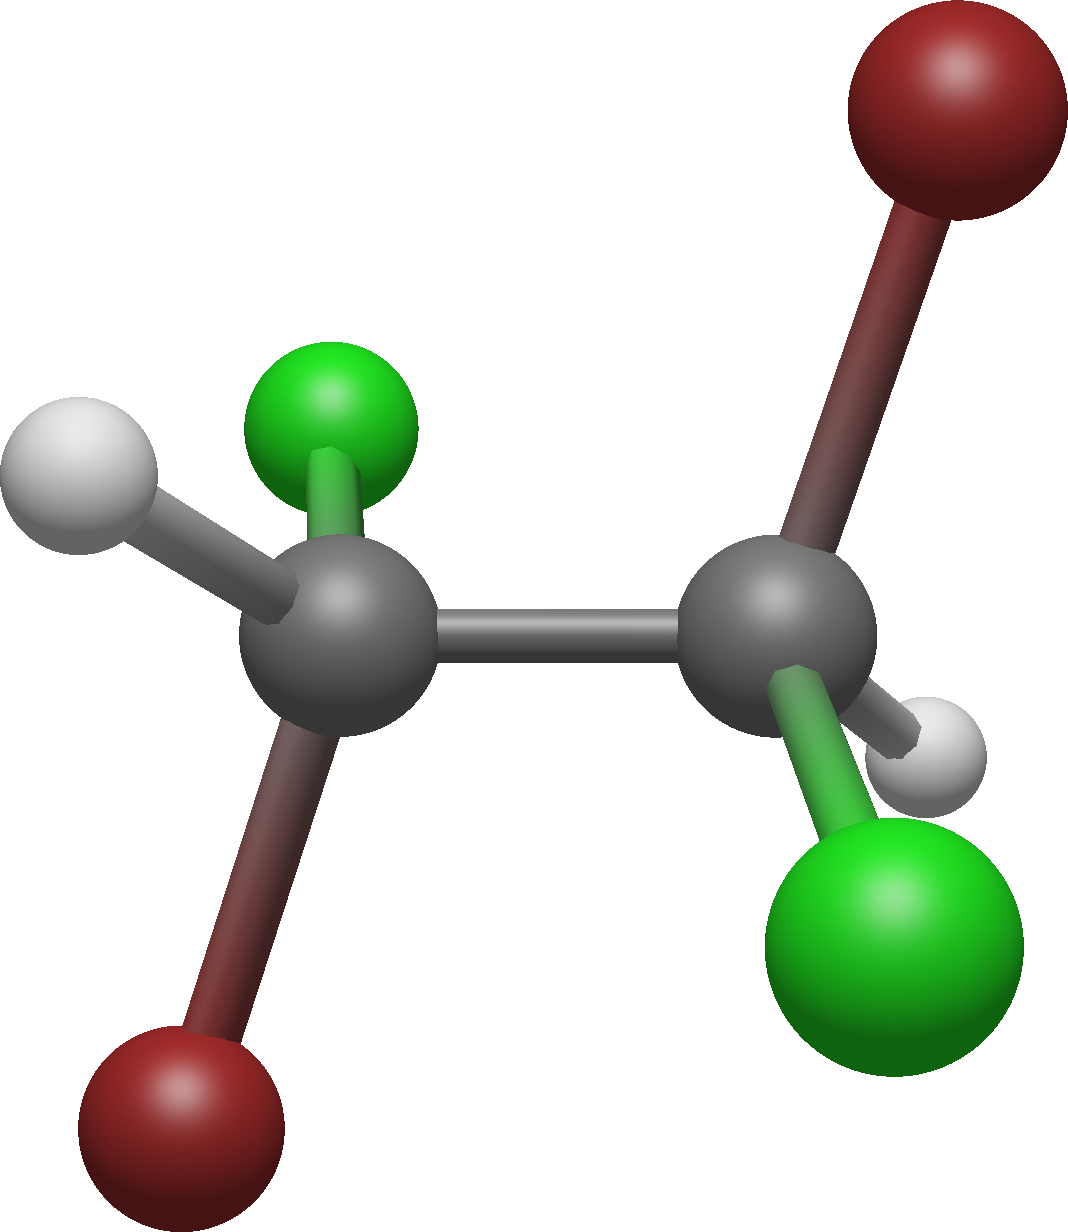
\includegraphics[width=1in]{figures/ciexample.png}\end{center}
    \end{frame}

    \begin{frame}{Point groups of high symmetry}
        Molecules in the $C_{\infty v}$ group are linear, with infinite rotation order and an infinite number of reflection planes containing the rotation axis. They contain no inversion center. An example is hydrogen chloride (\ch{HCl}).

        \begin{center}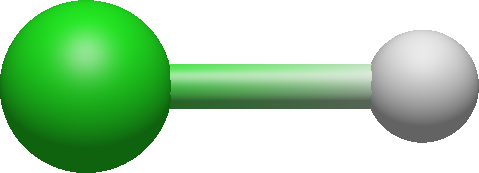
\includegraphics[width=1in]{figures/cinfvexample.png}\end{center}

        \onslide<2->
        {
            Molecules in the $D_{\infty h}$ group are like $C_{\infty v}$, but with perpendicular $C_2$ axes, a perpendicular mirror plane, and an inversion center. An example is carbon dioxide (\ch{CO2}).

            \begin{center}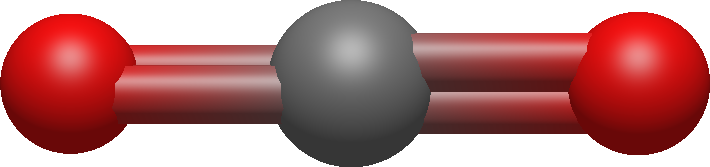
\includegraphics[width=1in]{figures/dinfhexample.png}\end{center}
        }
    \end{frame}

    \begin{frame}{Point groups of high symmetry}
        Molecules in the $T_d$ group are tetrahedral, with four $C_3$ axes, three $C_2$ axes, three $S_4$ axes, and six $\sigma_d$ mirror planes. An example is methane (\ch{CH4}).

        \begin{center}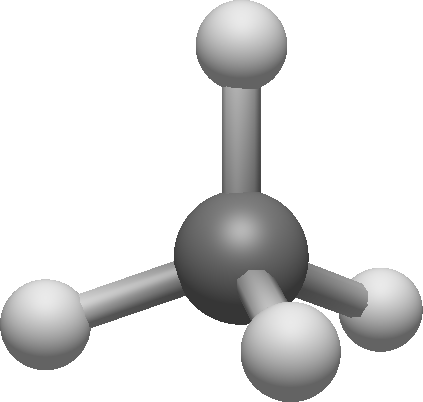
\includegraphics[width=1in]{figures/tdexample.png}\end{center}
    \end{frame}

    \begin{frame}{Point groups of high symmetry}
        Molecules in the $O_h$ group are octahedral, with 48 symmetry operations in all. An example is sulfur hexafluoride (\ch{SF6}).

        \begin{center}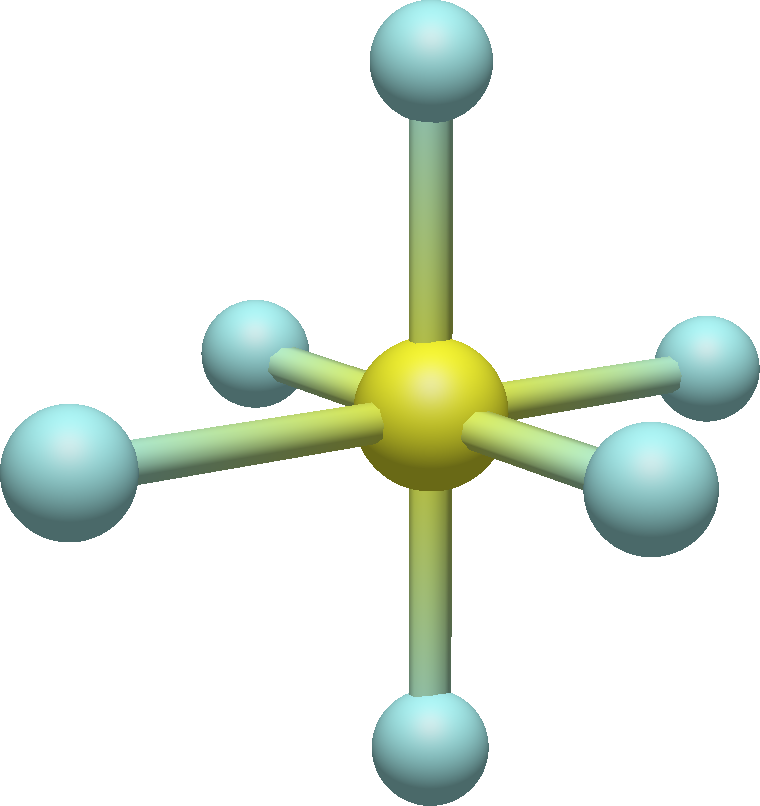
\includegraphics[width=1in]{figures/ohexample.png}\end{center}
    \end{frame}

    \begin{frame}{Point groups of high symmetry}
        Molecules in the $I_h$ group are icosahedral, with 120 symmetry operations in all. A fascinating example is buckminsterfullerene (\ch{C60}), a molecule with sixty carbon atoms in a ``soccer ball'' arrangement.
    
        \begin{center}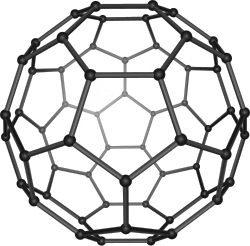
\includegraphics[width=1in]{figures/ihexample.png}\end{center}
    \end{frame}

    \begin{frame}{Other point groups}
        To distinguish which molecules are in each of the remaining point groups, we can refer to the flowchart provided in the handout.
        \vs
        
        Molecules in the $C_{nh}$ group contain a principal $C_n$ rotation axis and a horizontal mirror plane $\sigma_h$. The following examples are $C_{2h}$ (\emph{trans}-dinitrogen difluoride, \ch{N2F2}), $C_{2h}$ (1,5-dichloronaphthalene, \ch{C10H6Cl2}), and $C_{3h}$ (boric acid, \ch{H3BO3}), respectively:
    
        \begin{center}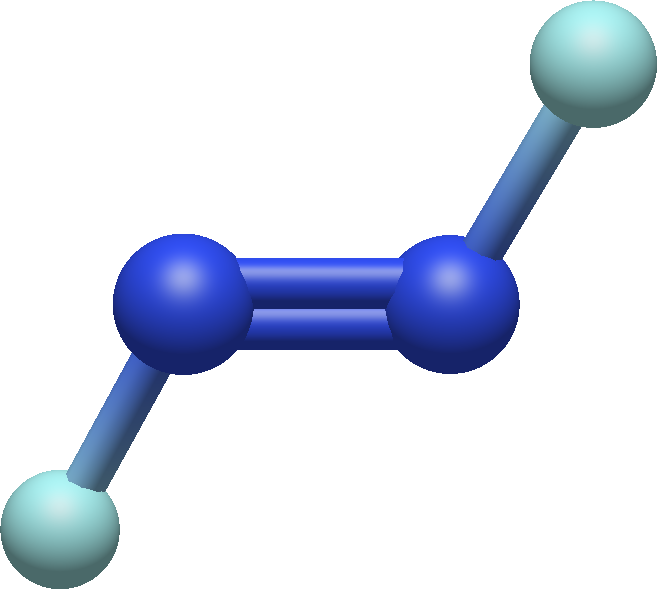
\includegraphics[width=1.2in]{figures/c2hexample1.png}\quad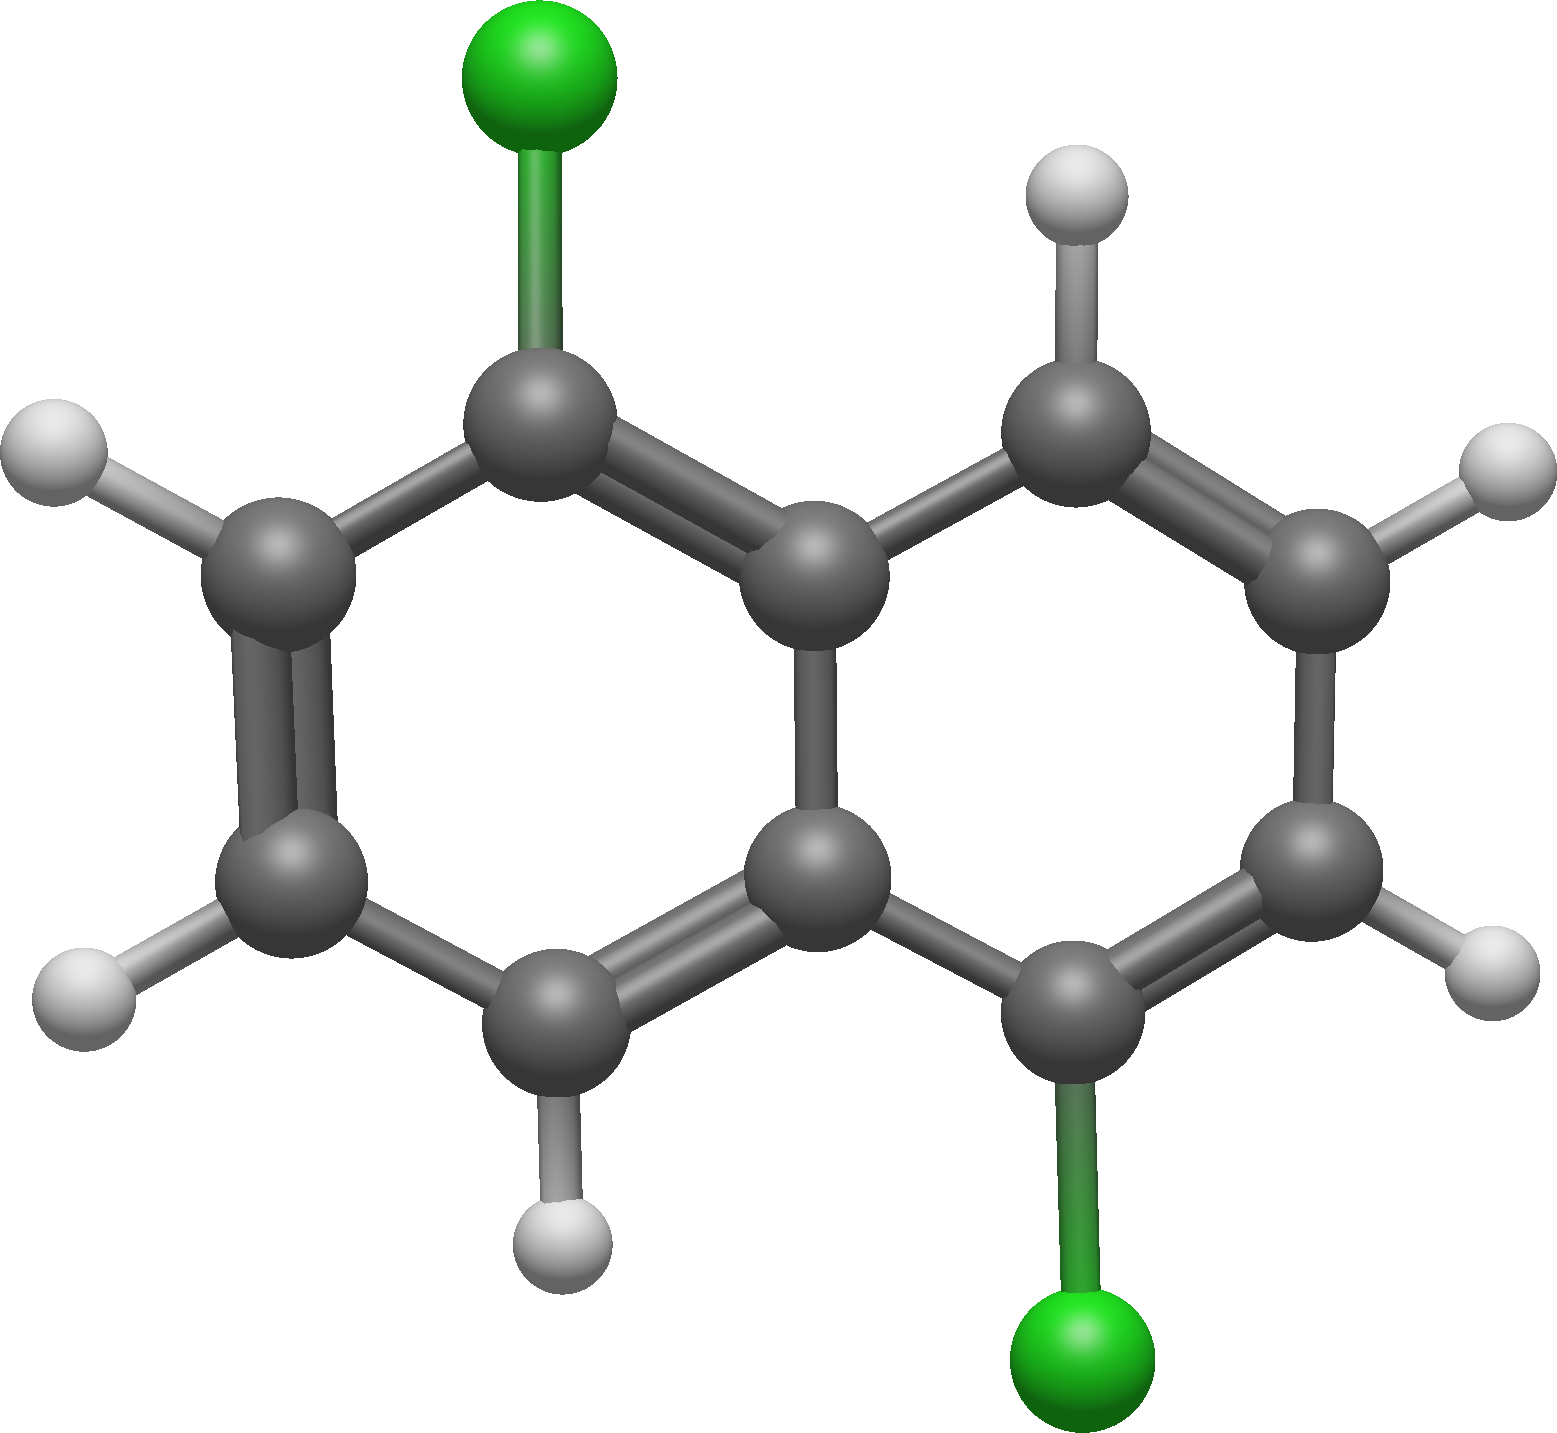
\includegraphics[width=1.2in]{figures/c2hexample2.png}\quad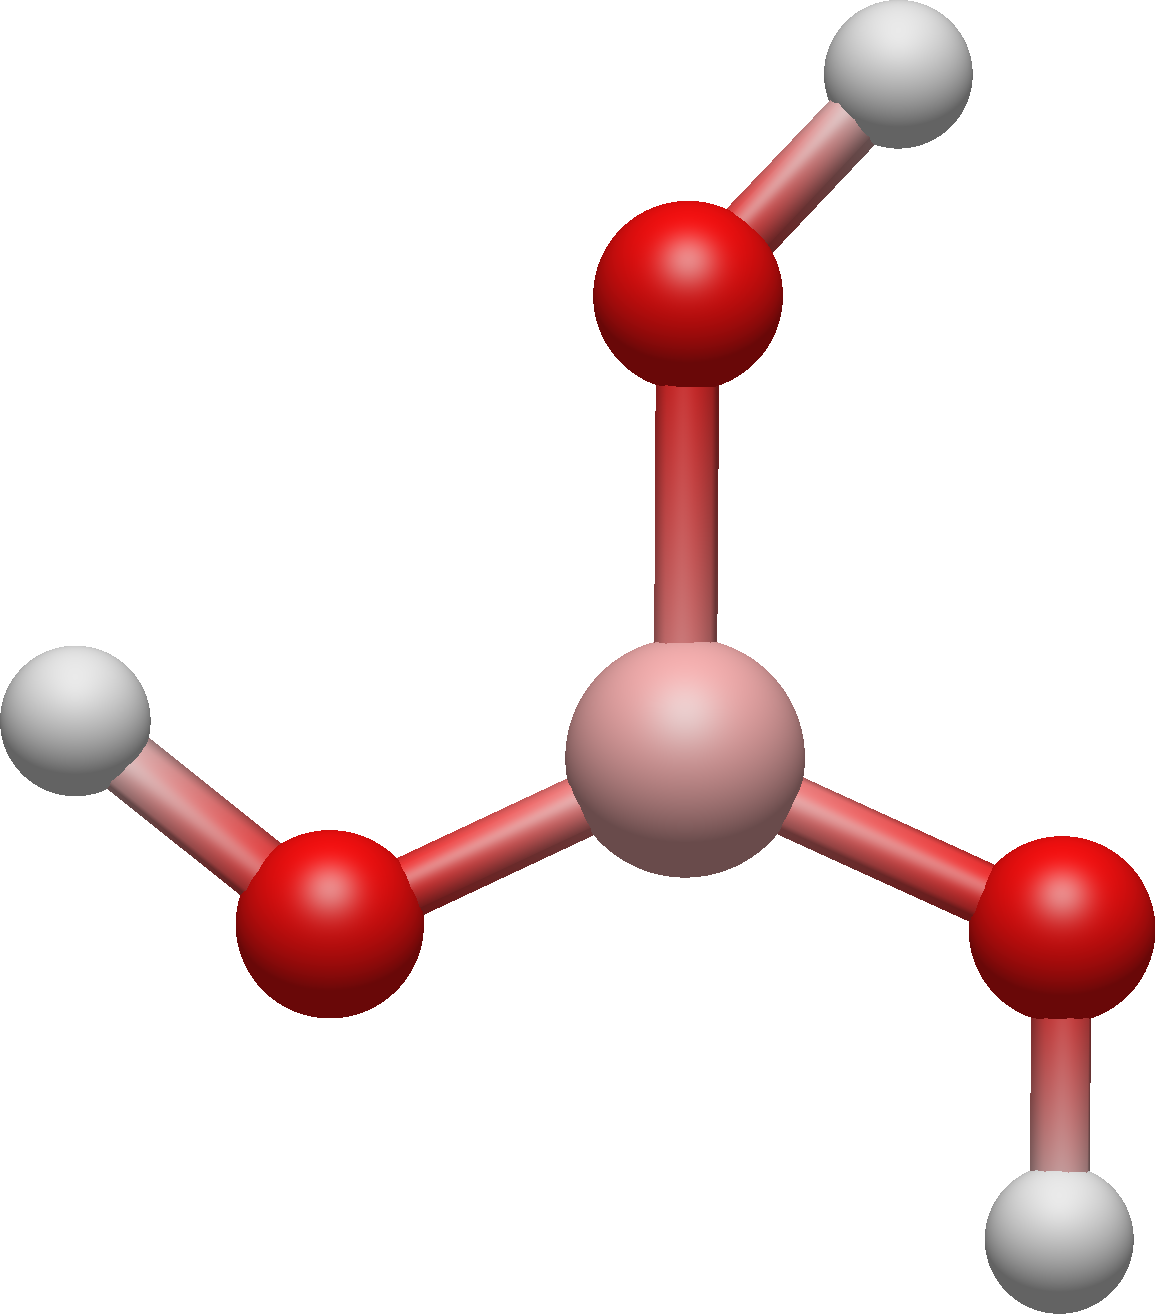
\includegraphics[width=1in]{figures/c3hexample.png}\end{center}
    \end{frame}

    \begin{frame}{Other point groups}
        Molecules in the $C_{nv}$ group contain a principal $C_n$ rotation axis and $n$ vertical mirror planes $\sigma_v$. The following examples are $C_{2v}$ (water, \ch{H2O}), $C_{3v}$ (ammonia, \ch{NH3}), and $C_{4v}$ (bromine pentafluoride, \ch{BrF5}), respectively:
    
        \begin{center}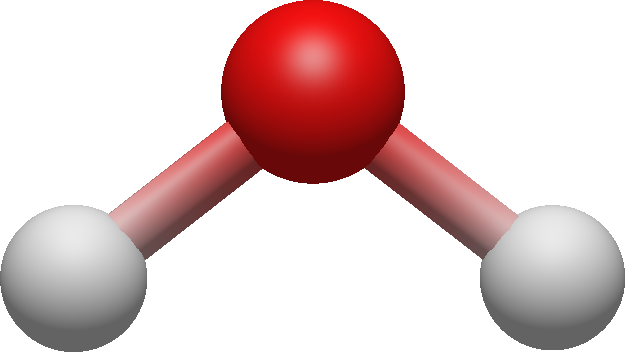
\includegraphics[width=1in]{figures/c2vexample.png}\quad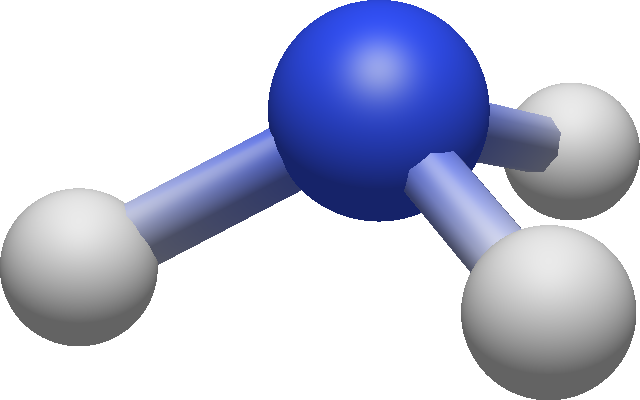
\includegraphics[width=1in]{figures/c3vexample.png}\quad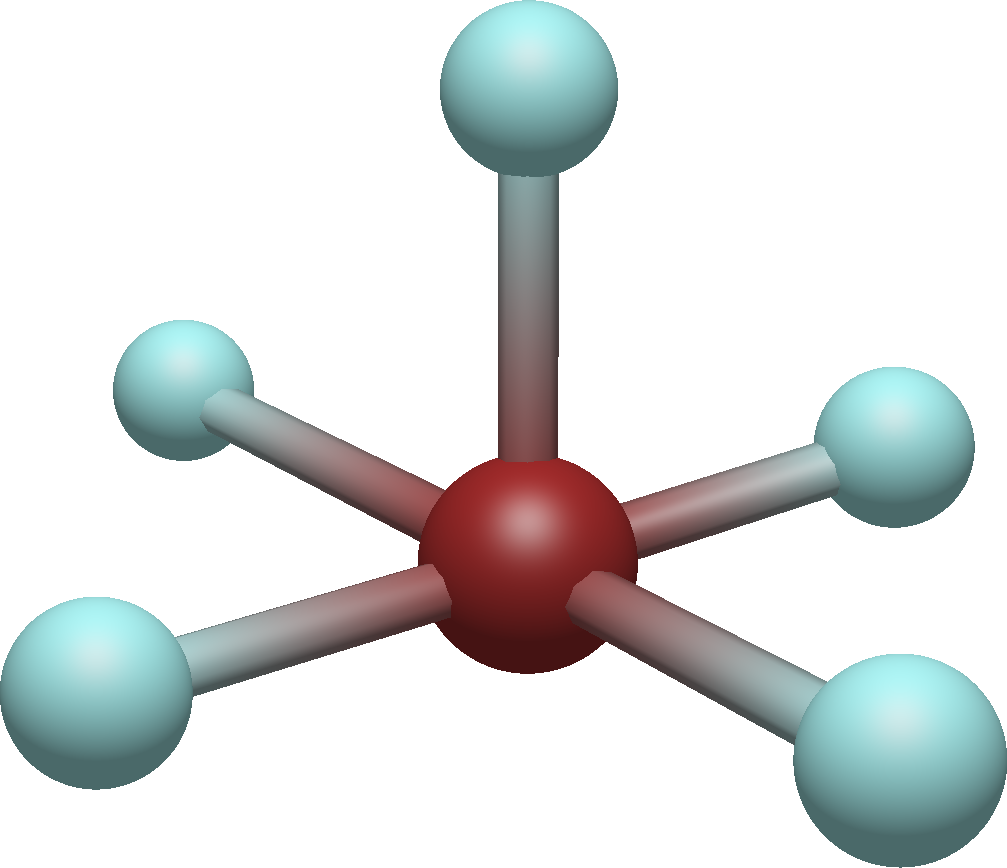
\includegraphics[width=1in]{figures/c4vexample.png}\end{center}
    \end{frame}

    \begin{frame}{Other point groups}
        Molecules in the $C_{n}$ group contain a principal $C_n$ rotation axis but no mirror planes. An example is hydrogen peroxide (\ch{H2O2}), which is in the point group $C_2$.
    
        \begin{center}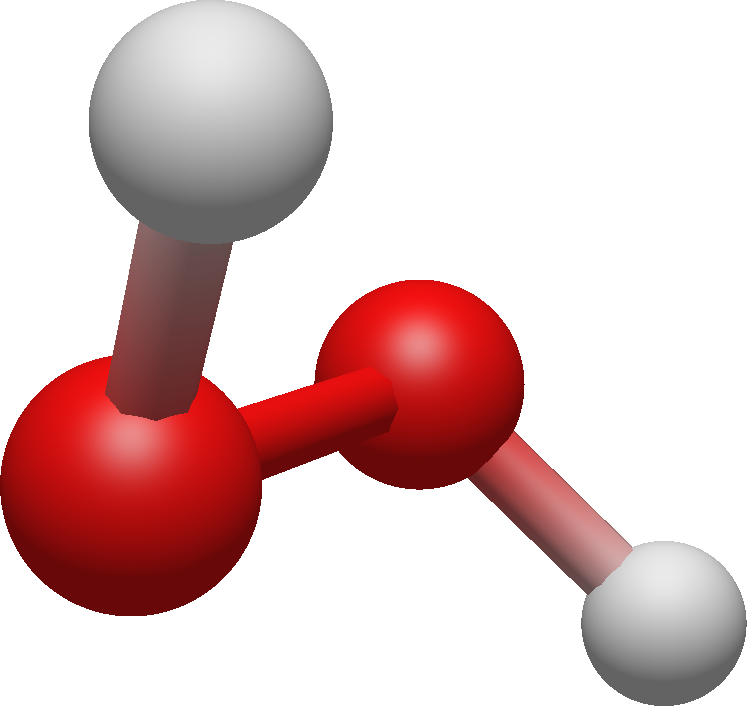
\includegraphics[width=0.9in]{figures/c2example.png}\end{center}
    \end{frame}

    \begin{frame}{Other point groups}
        Molecules in the $D_{nh}$ group contain a principal $C_n$ rotation axis and $n$ perpendicular $C_2$ rotation axes. They also have a horizontal mirror plane $\sigma_h$. The following examples are $D_{3h}$ (boron trifluoride, \ch{BF3}), $D_{3h}$ (phosphorus pentafluoride, \ch{PF5}), $D_{4h}$ (xenon tetrafluoride, \ch{XeF4}), and $D_{6h}$ (benzene, \ch{C6H6}), respectively:
    
        \begin{center}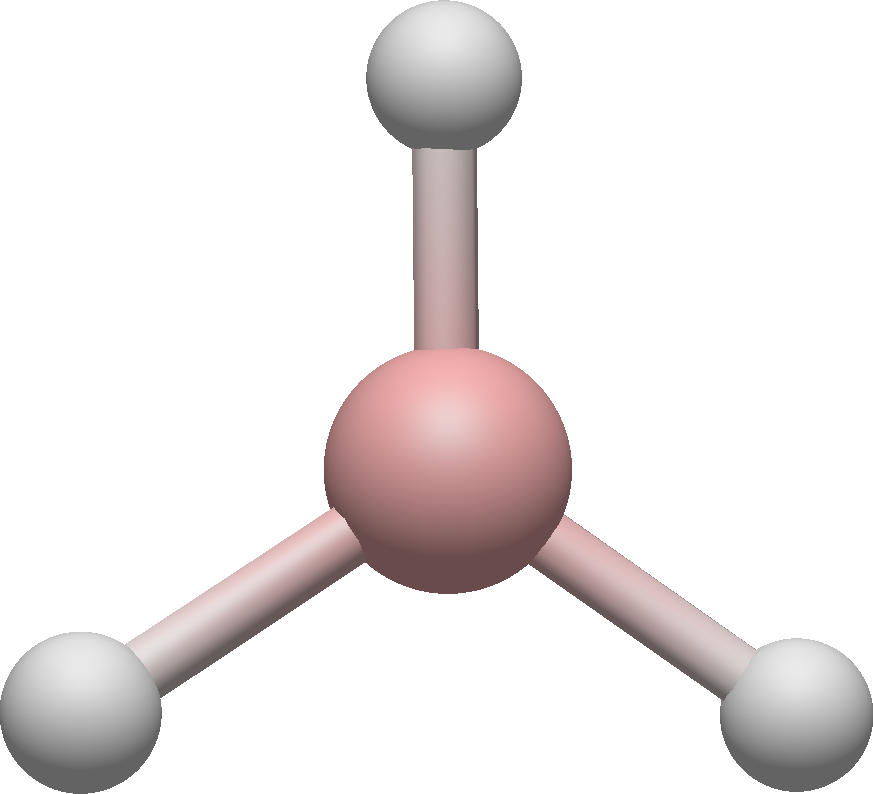
\includegraphics[width=1in]{figures/d3hexample1.png}\quad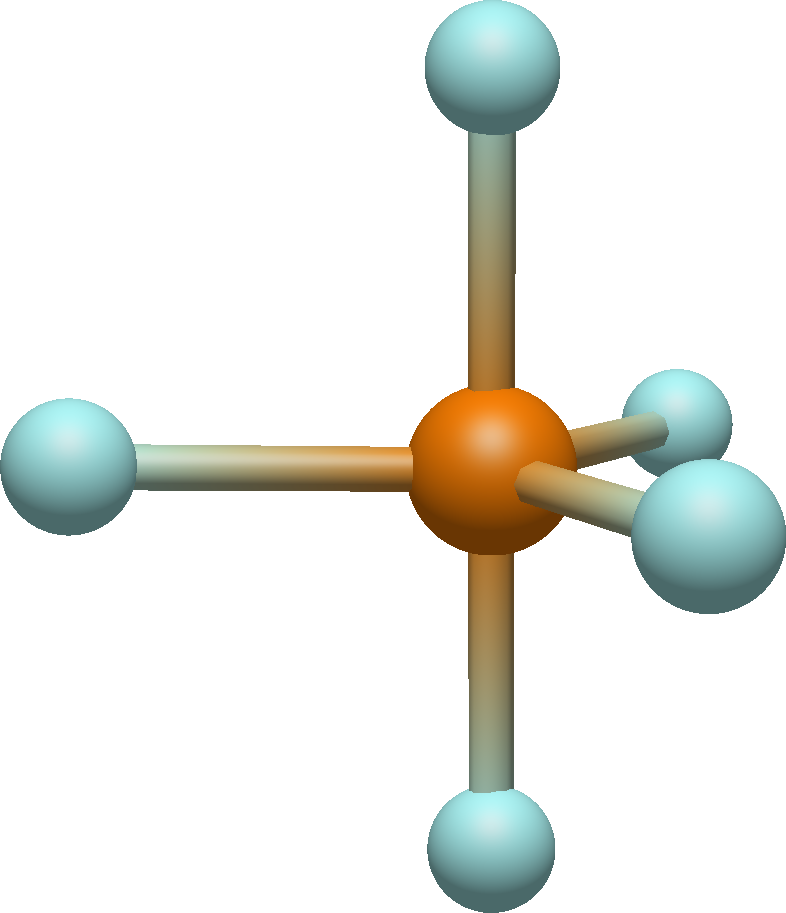
\includegraphics[width=0.8in]{figures/d3hexample2.png}\quad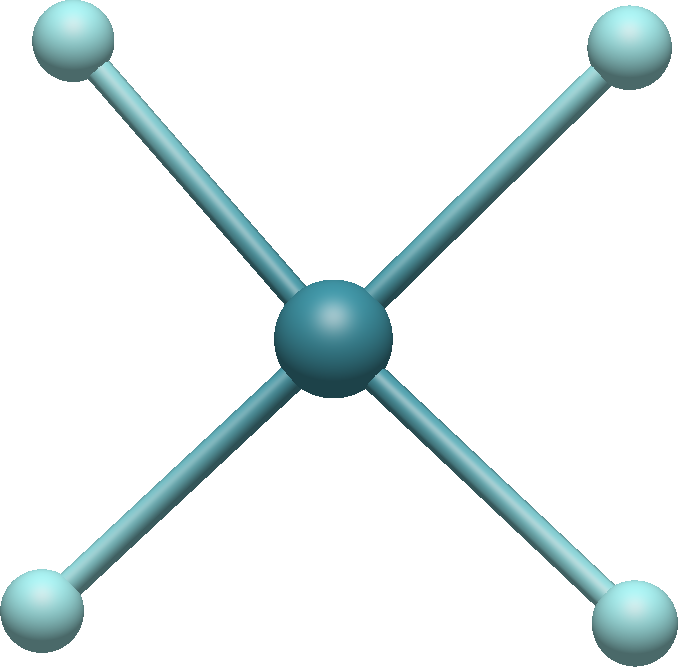
\includegraphics[width=1in]{figures/d4hexample.png}\quad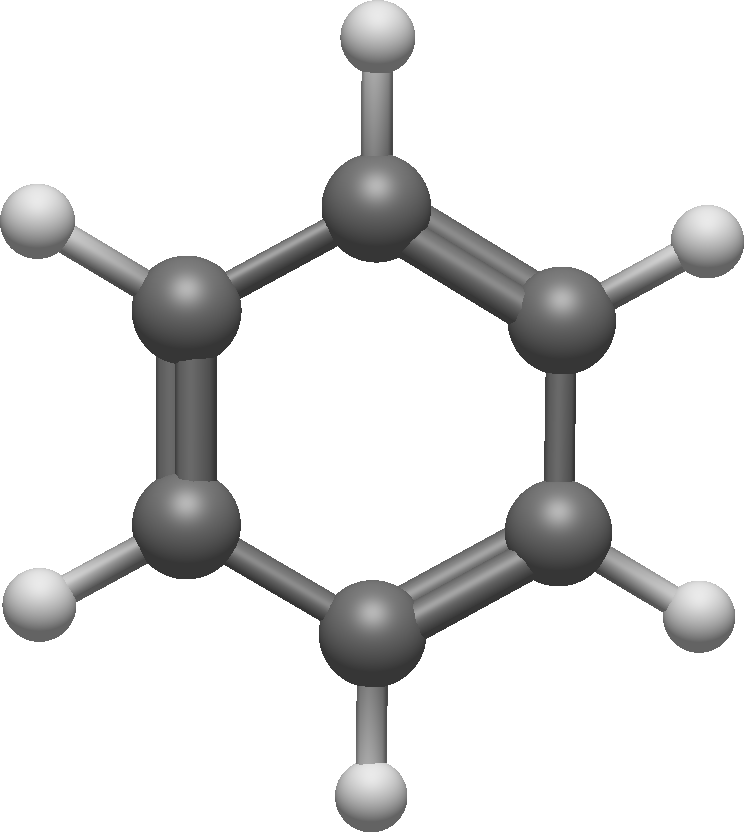
\includegraphics[width=1in]{figures/d6hexample.png}\end{center}
    \end{frame}

    \begin{frame}{Other point groups}
        Molecules in the $D_{nd}$ group contain a principal $C_n$ rotation axis and $n$ perpendicular $C_2$ rotation axes. They also have $n$ dihedral mirror planes $\sigma_d$. An example is ethane (\ch{C2H6}), which is in the point group $D_{3d}$.
        
        \begin{center}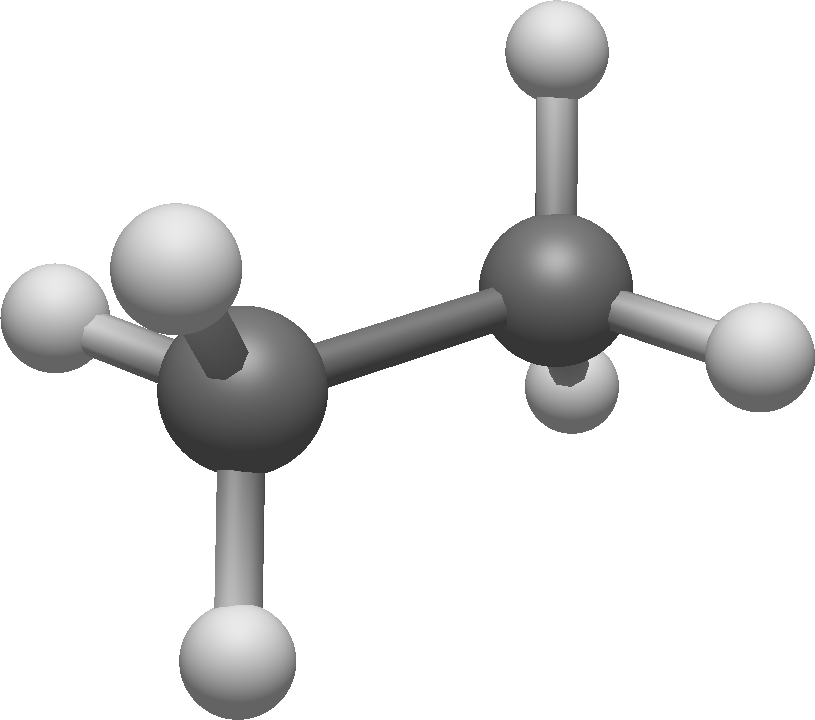
\includegraphics[width=1in]{figures/d3dexample.png}\end{center}
    \end{frame}

    \begin{frame}{Other point groups}
        Molecules in the $D_{n}$ group contain a principal $C_n$ rotation axis and $n$ perpendicular $C_2$ rotation axes, but no mirror planes. One interesting example of a $D_3$ molecule is the tris(ethylenediamine)cobalt(III) coordinate complex (\ch{[Co(en)3]^3+}, where \ch{en} = \ch{C2H8N2}). Look carefully at the geometry of the central cobalt atom (inset) and note the propeller shape.
        
        \begin{center}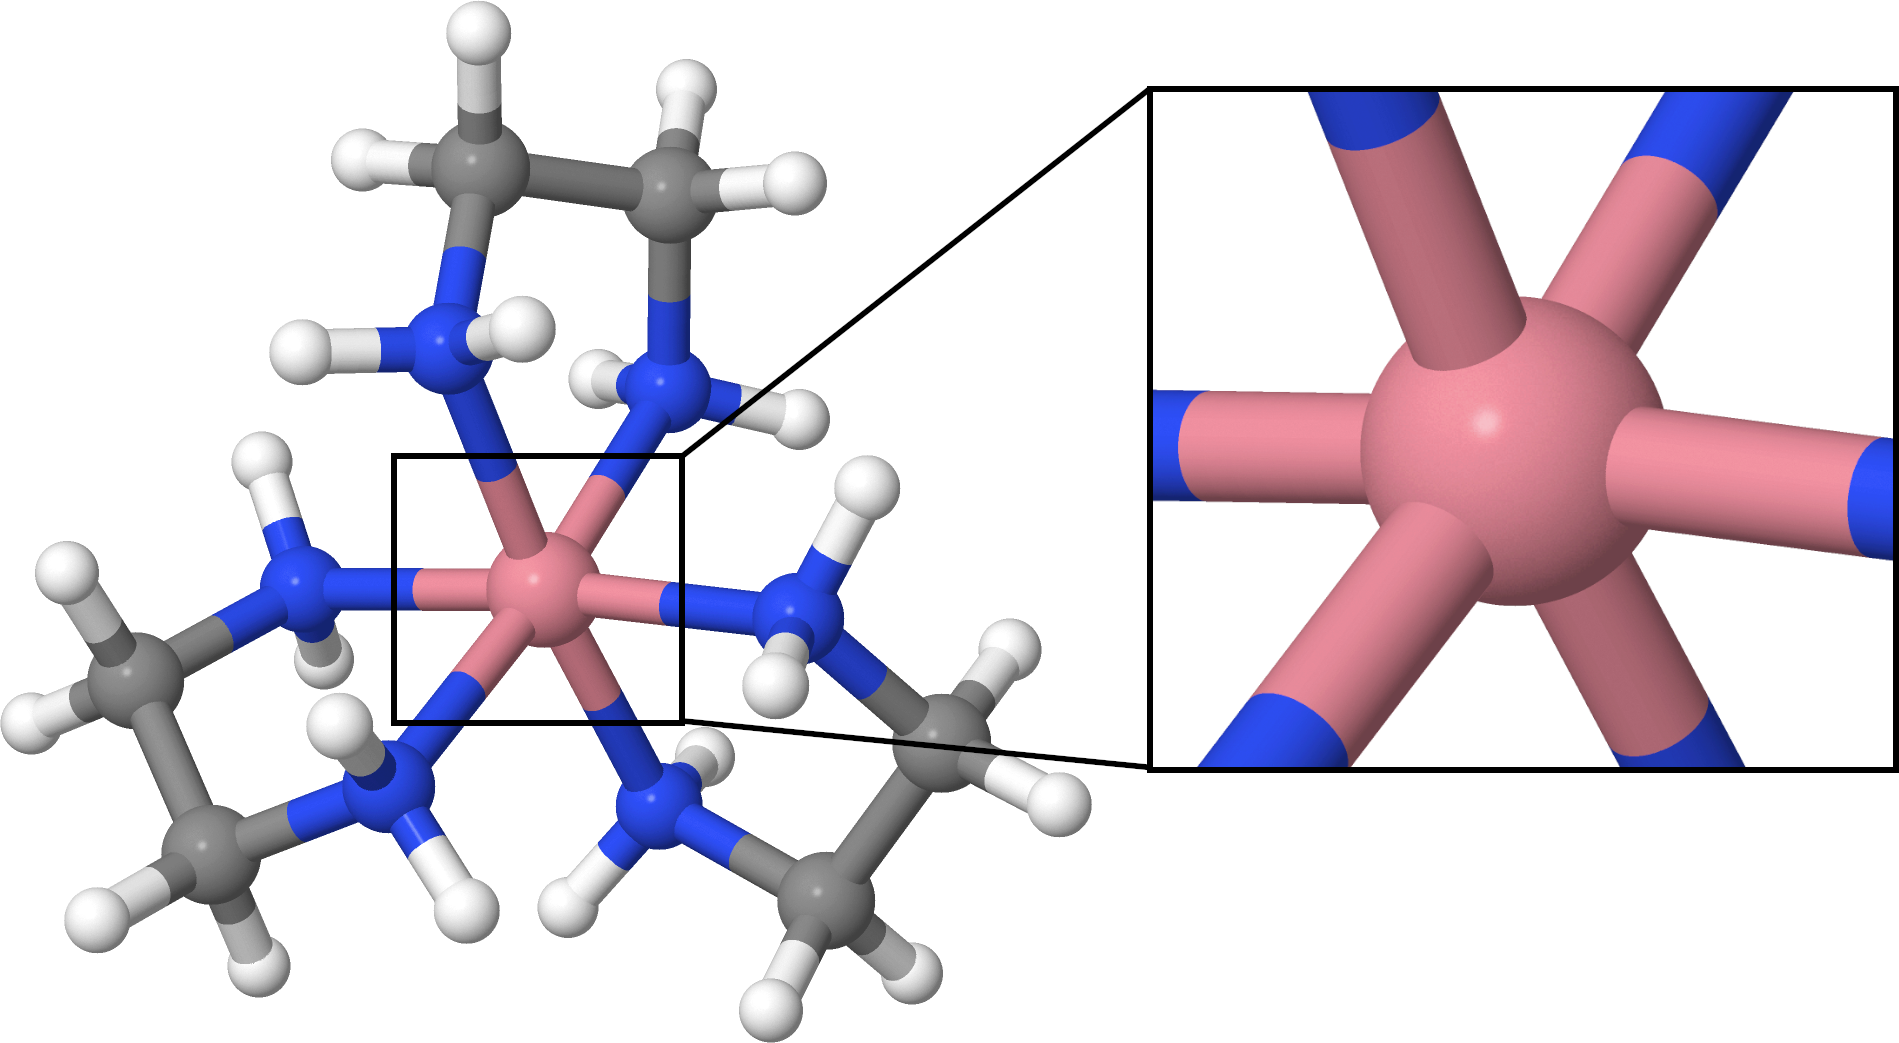
\includegraphics[width=0.75\linewidth]{figures/d3example.png}\end{center}
    \end{frame}

    \begin{frame}{Other point groups}
        Molecules are in the $S_{2n}$ group if they contain an $S_{2n}$ rotation-reflection axis, one principal $C_n$ rotation axis, and if they do not qualify to be in any of the $C$ or $D$ point groups. One molecule in the point group $S_4$ is 1,3,5,7-tetrafluorocyclooctatetraene (\ch{C8H4F4}), shown here from three different perspectives. Notice that the central carbon ring has an ``octagon boat'' shape.
    
        \begin{center}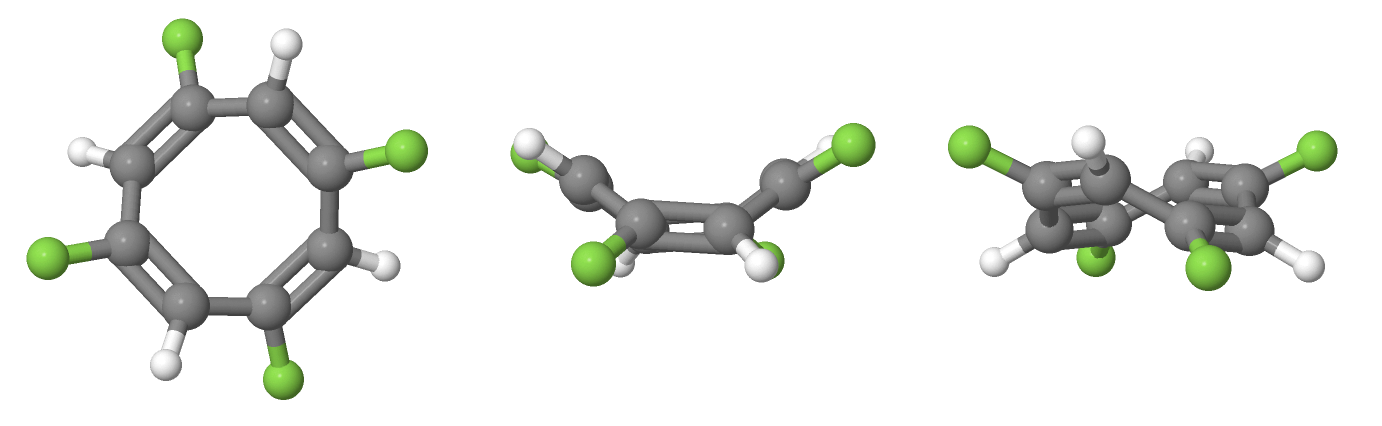
\includegraphics[width=\linewidth]{figures/s4example.png}\end{center}
    \end{frame}

    \section{\texorpdfstring{Algebraic structure of the point groups $C_{2v}$ and $C_{3v}$}{Algebraic structure of the point groups C2v and C3v}}

    \begin{frame}{Algebraic structure of the point groups $C_{2v}$ and $C_{3v}$}
        To understand point groups, we look at them using group theory. First, we verify that point groups are, indeed, groups. To illustrate, we will use the point groups of water (\ch{H2O}), $C_{2v}$, and ammonia (\ch{NH3}), $C_{3v}$, as examples.
        \vs

        \onslide<2->
        {
            First, we verify that $C_{2v}$ has an identity, inverses, closure, and associativity. Every point group, including $C_{2v}$, has an identity operation $E$. The $C_2$ rotation is its own inverse, as $C_2C_2=C_2^2=E$. The reflections $\sigma_{v1}$ and $\sigma_{v2}$ are their own inverses. Associativity follows from the associativity of function composition.
        }
    \end{frame}

    \begin{frame}{Algebraic structure of the point groups $C_{2v}$ and $C_{3v}$}
        The Cayley table for $C_{2v}$ is shown below. Closure can be verified. Furthermore, note that $C_{2v} \cong V_4$, and $C_{2v}$ is abelian.

        \begin{center}
            \renewcommand{\arraystretch}{1.5}
            \begin{tabular}{lr}
                \begin{tabular}{l}
                    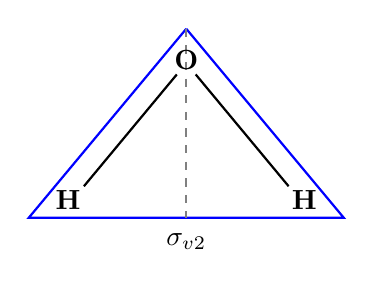
\begin{tikzpicture}[scale=2]
                        \coordinate (one) at (0,1.2);
                        \coordinate (two) at (1,0);
                        \coordinate (three) at (-1,0);
                        \coordinate (onetwo) at (0.5,0.866);
                        \coordinate (twothree) at (0,0);
                        \coordinate (onethree) at (-0.5,0.866);
                        \draw [blue,thick] (one)--(two)--(three)--(one);
                        \draw [gray,thick,dashed] (one)--(twothree);
                        \draw [black,thick,solid] (-0.06,0.91)--(-0.65,0.2);
                        \draw [black,thick,solid] (0.06,0.91)--(0.65,0.2);
                        \node at (0,-0.15) {$\sigma_{v2}$};
                        \node at (0,1) {\textbf O};
                        \node at (-0.75,0.11)
                        {\textbf H};
                        \node at (0.75,0.11)
                        {\textbf H};
                    \end{tikzpicture}\\
                    \begin{tabular}{l}
                        \scriptsize$E$: Identity\\
                        \scriptsize$C_2$: $180^{\circ}$\\
                        \scriptsize$\sigma_{v1}$: Reflection over molecular plane
                    \end{tabular}
                \end{tabular}
                &
                \begin{tabular}{cc|cccc}
                    & & \multicolumn{4}{c}{$g$}\\
                    & $f \circ g$ & $E$ & $C_2$ & $\sigma_{v1}$ & $\sigma_{v2}$\\
                    \hline
                    \multirow{4}{*}{$f$} & $E$ & $E$ & $C_2$ & $\sigma_{v1}$ & $\sigma_{v2}$\\
                    & $C_2$ & $C_2$ & $E$ & $\sigma_{v2}$ & $\sigma_{v1}$\\
                    & $\sigma_{v1}$ & $\sigma_{v1}$ & $\sigma_{v2}$ & $E$ & $C_2$\\
                    & $\sigma_{v2}$ & $\sigma_{v2}$ & $\sigma_{v1}$ & $C_2$ & $E$
                \end{tabular}
            \end{tabular}
        \end{center}
    \end{frame}

    \begin{frame}{Algebraic structure of the point groups $C_{2v}$ and $C_{3v}$}
        Now, we verify that $C_{3v}$ satisfies the definition of a group. Clearly, $C_{3v}$ has the identity operation $E$. The $C_3$ rotation has the inverse $C_3^2$. Likewise, $C_3^2$ has the inverse $C_3$. Each reflection $\sigma_{v}$ is its own inverse. Associativity follows from the associativity of function composition.
    \end{frame}

    \begin{frame}{Algebraic structure of the point groups $C_{2v}$ and $C_{3v}$}
        The Cayley table for $C_{3v}$ is shown below. Closure can be verified. Note that $C_{3v}\cong S_3$, and $C_{3v}$ is not abelian.

        \begin{center}
            \renewcommand{\arraystretch}{1.5}
            \begin{tabular}{lr}
                \begin{tabular}{l}
                    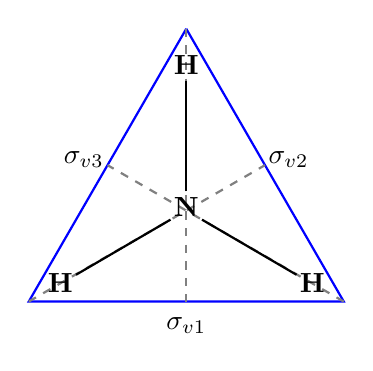
\begin{tikzpicture}[scale=2]
                        \coordinate (one) at (0,1.732);
                        \coordinate (two) at (1,0);
                        \coordinate (three) at (-1,0);
                        \coordinate (onetwo) at (0.5,0.866);
                        \coordinate (twothree) at (0,0);
                        \coordinate (onethree) at (-0.5,0.866);
                        \draw [blue,thick] (one)--(two)--(three)--(one);
                        \draw [gray,thick,dashed] (one)--(twothree);
                        \draw [gray,thick,dashed] (two)--(onethree);
                        \draw [gray,thick,dashed] (three)--(onetwo);
                        \draw [black,thick,solid] (0,0.7)--(0,1.4);
                        \draw [black,thick,solid] (-0.1,0.52)--(-0.7,0.17);
                        \draw [black,thick,solid] (0.1,0.52)--(0.7,0.17);
                        \node at (0,-0.15) {$\sigma_{v1}$};
                        \node at (0.65,0.9) {$\sigma_{v2}$};
                        \node at (-0.65,0.9)
                        {$\sigma_{v3}$};
                        \node at (0,0.6) {\textbf N};
                        \node at (0,1.5) {\textbf H};
                        \node at (-0.8,0.12) {\textbf H};
                        \node at (0.8,0.12) {\textbf H};
                    \end{tikzpicture}\\
                    \begin{tabular}{l}
                        \scriptsize$E$: Identity\\
                        \scriptsize\scriptsize$C_3$: $120^{\circ}$, counterclockwise\\
                        \scriptsize$C_3^2$: $240^{\circ}$, counterclockwise
                    \end{tabular}
                \end{tabular}
                &\footnotesize
                \begin{tabular}{cc|cccccc}
                    & & \multicolumn{6}{c}{$g$}\\
                    & $f \circ g$ & $E$ & $C_3$ & $C_3^2$ & $\sigma_{v1}$ & $\sigma_{v2}$ & $\sigma_{v3}$\\
                    \hline
                    \multirow{6}{*}{$f$} & $E$ & $E$ & $C_3$ & $C_3^2$ & $\sigma_{v1}$ & $\sigma_{v2}$ & $\sigma_{v3}$\\
                    & $C_3$ & $C_3$ & $C_3^2$ & $E$ & $\sigma_{v3}$ & $\sigma_{v1}$ & $\sigma_{v2}$\\
                    & $C_3^2$ & $C_3^2$ & $E$ & $C_3$ & $\sigma_{v2}$ & $\sigma_{v3}$ & $\sigma_{v1}$\\
                    & $\sigma_{v1}$ & $\sigma_{v1}$ & $\sigma_{v2}$ & $\sigma_{v3}$ & $E$ & $C_3$ & $C_3^2$\\
                    & $\sigma_{v2}$ & $\sigma_{v2}$ & $\sigma_{v3}$ & $\sigma_{v1}$ & $C_3^2$ & $E$ & $C_3$\\
                    & $\sigma_{v3}$ & $\sigma_{v3}$ & $\sigma_{v1}$ & $\sigma_{v2}$ & $C_3$ & $C_3^2$ & $E$
                \end{tabular}
            \end{tabular}
        \end{center}
    \end{frame}

    \begin{frame}{Matrix representation of symmetry operations}
        Let $\mathcal B$ represent the standard ordered basis of $\mathbb{R}^3$.
        \vs

        We can express the matrix representation of $C_{2v}$ and $C_{3v}$. We will look at $C_{2v}$ (water, \ch{H2O}) first. These matrices will be with respect to the basis $\mathcal B$.
        \vs

        \onslide<2->
        {
            By convention, we set the $z$ axis as the principal axis and the $xz$ plane as the plane of the molecule, with the oxygen atom at the origin, as shown:

            \begin{center}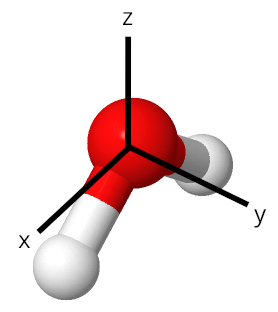
\includegraphics[width=1.25in]{figures/waterxyz.png}\end{center}
        }
    \end{frame}

    \begin{frame}{Matrix representation of symmetry operations}
        The matrices for the symmetry operations of $C_{2v}$ are \[M_E=\begin{bmatrix}1&0&0\\0&1&0\\0&0&1\end{bmatrix}, M_{C_2}=\begin{bmatrix}-1&0&0\\0&-1&0\\0&0&1\end{bmatrix},\]\[M_{\sigma_{v1}}=\begin{bmatrix}1&0&0\\0&-1&0\\0&0&1\end{bmatrix}, \text{ and } M_{\sigma_{v2}}=\begin{bmatrix}-1&0&0\\0&1&0\\0&0&1\end{bmatrix}.\]\vs
        
        Multiplying these matrices reveals the same group structure as shown in the Cayley table.
    \end{frame}

    \begin{frame}{Matrix representation of symmetry operations}
        Now we will look at $C_{3v}$ (ammonia, \ch{NH3}). These matrices will be with respect to the basis $\mathcal B$. By convention, we set the $z$ axis as the principal axis, the $xy$ plane as parallel to the hydrogen triangle, and the $xz$ plane coinciding with one of the three $\sigma_v$ mirror planes, with the nitrogen atom at the origin, as shown:
    
        \begin{center}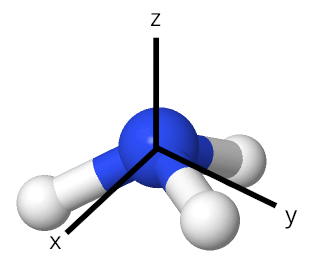
\includegraphics[width=1.5in]{figures/ammoniaxyz.png}\end{center}
    \end{frame}

    \begin{frame}{Matrix representation of symmetry operations}
        The matrices for the symmetry operations of $C_{3v}$ are \[M_E=\begin{bmatrix}1&0&0\\0&1&0\\0&0&1\end{bmatrix}, M_{C_3}=\begin{bmatrix}-\frac12&-\frac{\sqrt{3}}2&0\\\frac{\sqrt{3}}2&-\frac12&0\\0&0&1\end{bmatrix},\]\[M_{C_3^2}=\begin{bmatrix}-\frac12&\frac{\sqrt{3}}2&0\\-\frac{\sqrt{3}}2&-\frac12&0\\0&0&1\end{bmatrix},M_{\sigma_{v1}}=\begin{bmatrix}1&0&0\\0&-1&0\\0&0&1\end{bmatrix},\]\[M_{\sigma_{v2}}=\begin{bmatrix}-\frac12&-\frac{\sqrt{3}}2&0\\-\frac{\sqrt3}2&\frac12&0\\0&0&1\end{bmatrix}, \text{ and } M_{\sigma_{v3}}=\begin{bmatrix}-\frac12&\frac{\sqrt{3}}2&0\\\frac{\sqrt3}2&\frac12&0\\0&0&1\end{bmatrix}.\]\vs
        
        Multiplying these matrices reveals the same group structure as shown in the Cayley table.
    \end{frame}

    \section{Characters and irreducible representations}

    \begin{frame}{Mulliken symbols}
        We want to decompose the representations into irreducible representations (irreps). The irreps will be denoted using a standard notation system, called Mulliken symbols. \cite{mulliken1955}\vs

        \onslide<2->
        {
            $A$: 1D irrep, symmetric (character $1$) w.r.t. principal rotation\\
            $B$: 1D irrep, antisymmetric (character $-1$) w.r.t. principal rotation\\
            $E$: 2D irrep\\
            $T$: 3D irrep
        }

        \onslide<3->
        {
            Subscript 1: symmetric w.r.t. perpendicular $C_2$ axis\\
            Subscript 2: antisymmetric w.r.t. perpendicular $C_2$ axis\\
            (If no perpendicular $C_2$ axis, subscript 1 or 2 is based on symmetry/antisymmetry w.r.t. $\sigma_v$ mirror plane)\\
            Subscript $g$ (\emph{gerade}): symmetric w.r.t. inversion $i$\\
            Subscript $u$ (\emph{ungerade}): antisymmetric w.r.t. inversion $i$
            \\
            $'$ (\emph{single prime}): symmetric w.r.t. $\sigma_h$ mirror plane\\
            $''$ (\emph{double prime}): antisymmetric w.r.t. $\sigma_h$ mirror plane
        }
    \end{frame}
    
    \begin{frame}{Properties of character tables}
        Character tables provide all symmetry information in a succinct manner. Tables for a large number of common point groups are readily available for reference. We will construct tables for $C_{2v}$ and $C_{3v}$. Before starting, we will consider a list of properties that character tables exhibit. \cite{miessler2014,mcgrady2024,serre}
        \vs

        \onslide<2->
        {
            Let $G$ be a point group. Let $\Gamma$ be a reducible representation of $G$. Let $\Gamma^{(i)}$ be an irreducible representation (irrep) of $G$. Let $\chi^{(i)}(C)$ represent the character of conjugacy class $C$ in the irrep $\Gamma^{(i)}$.
        }

        \onslide<3->
        {
            \begin{enumerate}
                \item The number of symmetry operations is $|G|$, the order of the group.
                \item If symmetry operations are grouped by conjugacy class $C$, we show how many operations are in the class, $n_C$, in the top row. For example, if there are three rotations in the $C_2$ class, the top row will be labeled $3C_2$. We will call $n_C$ the multiplicity of the class.
            \end{enumerate}
        }
    \end{frame}

    \begin{frame}{Properties of character tables}
        \begin{enumerate}
            \setcounter{enumi}{2}
            \item The number of irreps equals the number of classes. That is, the character table needs to have the same number of rows and columns.
            \item Taking the sum over all of the irreps, we have \[\sum_i\chi^{(i)}(E)\overline{\chi^{(i)}(E)}=|G|,\] where $E$ is the identity operation.
            \item For the irrep $\Gamma^{(i)}$, we have \begin{equation}\sum_C n_C \chi^{(i)}(C)\overline{\chi^{(i)}(C)}=|G|,\label{eq:sumsq}\end{equation} where the sum is taken over all of the conjugacy classes.
        \end{enumerate}
    \end{frame}

    \begin{frame}{Properties of character tables}
        \begin{enumerate}
            \setcounter{enumi}{5}
            \item \label{property:orthogonality} Characters of irreducible representations are orthogonal. We have, for the irreps $\Gamma^{(i)}$ and $\Gamma^{(j)}$, \begin{equation}
            \sum_C n_C \chi^{(i)}(C)\overline{\chi^{(j)}(C)}=|G|\delta_{ij},\label{eq:orthog}\end{equation} where $\delta_{ij}$ is the Kronecker delta. This form follows from the standard orthogonality relations for characters, together with the fact that characters are constant on conjugacy classes. When $i=j$, \eqref{eq:orthog} reduces to \eqref{eq:sumsq}, and when $i\neq j$, we have \[\sum_C n_C \chi^{(i)}(C)\overline{\chi^{(j)}(C)}=0.\]
            \item One irrep has characters that are all $1$, which is labeled $A_1$.
            \item Each irrep must be distinct.
            \item The character for the identity operation $E$ is a positive integer for every irrep, equal to the dimension of the irrep.
        \end{enumerate}
    \end{frame}

    \begin{frame}{Properties of character tables}
        To construct the character table for $C_{2v}$, recall that the representation matrices of $C_{2v}$ found previously, with respect to the basis $\mathcal B$, are in block-diagonal form with $1\times 1$ blocks (i.e., diagonal form), and here we visually identify the blocks with color-coded boxes.
        \vs

        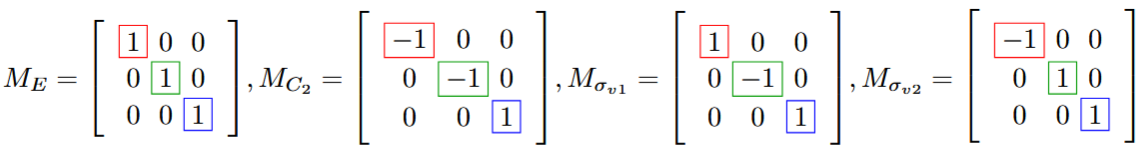
\includegraphics[width=1\linewidth]{figures/colorcodematricesc2v.png}
    \end{frame}

    \begin{frame}{Properties of character tables}
        We start building a character table by placing the traces of the first blocks in the first row ($x$), the traces of the second blocks in the second row ($y$), and the traces of the third blocks in the third row ($z$). The rows are color-coded to match their corresponding blocks. Of course, the trace of a $1\times 1$ block is a single element.
    
        \begin{table}[htbp]
            \centering
            \renewcommand{\arraystretch}{1.5}
            \begin{tabular}{c|cccc}
                $C_{2v}$ & $E$ & $C_2$ & $\sigma_{v1}$ & $\sigma_{v2}$\\
                \hline
                \color{red}$(x)$ & \color{red}$1$ & \color{red}$-1$ & \color{red}$1$ & \color{red}$-1$\\
                \color{green!60!black}$(y)$ & \color{green!60!black}$1$ & \color{green!60!black}$-1$ & \color{green!60!black}$-1$ & \color{green!60!black}$1$\\
                \color{blue}$(z)$ & \color{blue}$1$ & \color{blue}$1$ & \color{blue}$1$ & \color{blue}$1$
            \end{tabular}
        \end{table}
    \end{frame}

    \begin{frame}{Properties of character tables}
        Since $C_{2v}$ has four conjugacy classes, rule 3 tells us that there must be four irreps. Applying rules 6, 8, and 9, we find the characters of the fourth irrep. We now label the rows by the Mulliken symbols $A_1$, $A_2$, $B_1$, and $B_2$ by the aforementioned rules, and we sort the rows by the Mulliken symbols.
    
        \begin{table}[htbp]
            \centering
            \renewcommand{\arraystretch}{1.5}
            \begin{tabular}{c|cccc}
                $C_{2v}$ & $E$ & $C_2$ & $\sigma_{v1}$ & $\sigma_{v2}$\\
                \hline
                $A_1$ & $1$ & $1$ & $1$ & $1$\\
                $A_2$ & $1$ & $1$ & $-1$ & $-1$\\
                $B_1$ & $1$ & $-1$ & $1$ & $-1$\\
                $B_2$ & $1$ & $-1$ & $-1$ & $1$\\
            \end{tabular}
        \end{table}
        
        We now have a complete character table for $C_{2v}$.
    \end{frame}

    \begin{frame}{Properties of character tables}
        To construct the character table for $C_{3v}$, recall that the representation matrices for $C_{3v}$ found previously, with respect to the basis $\mathcal B$, are in block-diagonal form. Note that we need each matrix to have the same block sizes. Since the $C_{3v}$ matrices are not all diagonal, we need $2\times2$ and $1\times1$ blocks so that every nonzero element is within a block and that the blocks are as small as possible. Here we visually identify the blocks with color-coded boxes.

        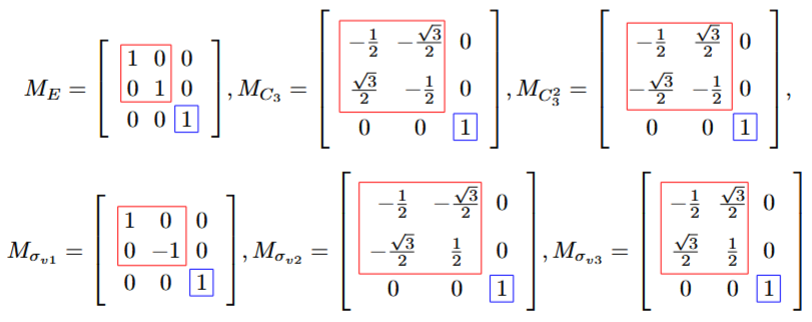
\includegraphics[width=\linewidth]{figures/colorcodematricesc3v.png}
    \end{frame}

    \begin{frame}{Properties of character tables}
        We start building a character table by placing the traces of the first blocks in the first row ($x, y$) and the traces of the second block in the second row ($z$). The $C_3$ and $C_3^2$ operations are in the same conjugacy class, and likewise the three $\sigma_v$ operations are in the same class, so they are grouped together. The rows are color-coded to match their corresponding blocks.

        \begin{table}[htbp]
            \centering
            \renewcommand{\arraystretch}{1.5}
            \begin{tabular}{c|ccc}
                $C_{3v}$ & $E$ & $2C_3$ & $3\sigma_{v}$\\
                \hline
                \color{red}$(x,y)$ & \color{red}$2$ & \color{red}$-1$ & \color{red}$0$\\
                \color{blue}$(z)$ & \color{blue}$1$ & \color{blue}$1$ & \color{blue}$1$
            \end{tabular}
        \end{table}
    \end{frame}

    \begin{frame}{Properties of character tables}
        Since $C_{3v}$ has three conjugacy classes, rule 3 tells us that there must be three irreps. Applying rules 6, 8, and 9, we find the characters of the third irrep. We now label the rows by the Mulliken symbols $A_1$, $A_2$, and $E$ by the aforementioned rules, and we sort the rows by the Mulliken symbols.
        
        \begin{table}[htbp]
            \centering
            \renewcommand{\arraystretch}{1.5}
            \begin{tabular}{c|ccc}
                $C_{3v}$ & $E$ & $2C_3$ & $3\sigma_{v}$\\
                \hline
                $A_1$ & $1$ & $1$ & $1$\\
                $A_2$ & $1$ & $1$ & $-1$\\
                $E$ & $2$ & $-1$ & $0$\\
            \end{tabular}
        \end{table}

        We now have a complete character table for $C_{3v}$.
    \end{frame}

    \begin{frame}{Properties of character tables}
        \begin{table}[htbp]
            \centering
            \renewcommand{\arraystretch}{1.5}
            \begin{tabular}{c|ccc}
                $C_{3v}$ & $\boxed{E}$ & $2C_3$ & $3\sigma_{v}$\\
                \hline
                $A_1$ & $1$ & $1$ & $1$\\
                $A_2$ & $1$ & $1$ & $-1$\\
                $\boxed{E}$ & $2$ & $-1$ & $0$\\
            \end{tabular}
        \end{table}
    
        Notice that the character table has a row labeled $E$ for the 2D irrep and a column labeled $E$ for the identity operation. This is confusing, but it is the convention used for character tables in chemistry.
        \vs

        \onslide<2->
        {
            Quirks like this almost led me to naming my project ``Why mathematicians and chemists don't understand each other.''
        }
    \end{frame}

    \section{\texorpdfstring{Eigenvalues of representations of $C_{2v}$ and $C_{3v}$}{Eigenvalues of representations of C2v and C3v}}
    
    \begin{frame}{Eigenvalues of representations of $C_{2v}$ and $C_{3v}$}
        We note that all of the characters we have found so far are in the integer set $\{-1,0,1,2\}$. At this point, we may ask if there are point groups for which other integers appear as characters, or indeed if there are point groups with non-integer characters.
        \vs
        
        \onslide<2->
        {
            To begin investigating, we will do some linear algebra on the symmetry operation matrices for $C_{2v}$ and $C_{3v}$. In particular, we find their characteristic polynomials, eigenvalues, and minimal polynomials. Surprisingly, this opens the door to cyclotomic field structures and Galois actions, which will reveal some of the algebraic number theory behind the characters.
        }
        \vs

        \onslide<3->
        {
            In the discussion that follows, for a square matrix $A$, we will denote the characteristic polynomial of $A$ as $p_A(x)$ and the minimal polynomial of $A$ as $m_A(x)$. We will denote the $n$th cyclotomic polynomial as $\Phi_n(x)$.
        }
    \end{frame}
    
    \begin{frame}{Eigenvalues of representations of $C_{2v}$ and $C_{3v}$}
        \begin{table}[p]
            \centering
            \renewcommand{\arraystretch}{3}
            \begin{tabular}{cccc}
                Matrix $M_i$ & $p_{M_i}(x)$ & Evals. (alg. mult.) & $m_{M_i}(x)$\\
                \hline
                $M_E$ & $(x-1)^3$ & $1$ (3) & $\Phi_1(x)$\\[5mm]
                $M_{C_2}$ & $(x-1)(x+1)^2$ & $1$ (1), $-1$ (2) & $\Phi_1(x)\Phi_2(x)$\\[5mm]
                $M_{\sigma_{v1}}, M_{\sigma_{v2}}$ & $(x-1)^2(x+1)$ & $1$ (2), $-1$ (1) & $\Phi_1(x)\Phi_2(x)$
            \end{tabular}
            \caption{Characteristic polynomials, eigenvalues (and their algebraic multiplicities), and minimal polynomials for the matrices in the point group $C_{2v}$.}
        \end{table}
    \end{frame}

    \begin{frame}{Eigenvalues of representations of $C_{2v}$ and $C_{3v}$}
        \begin{table}[htbp]
            \centering\small
            \renewcommand{\arraystretch}{3}
            \begin{tabular}{cccc}
                Matrix $M_i$ & $p_{M_i}(x)$ & Evals. (alg. mult.) & $m_{M_i}(x)$\\
                \hline
                $M_E$ & $(x-1)^3$ & $1$ (3) & $\Phi_1(x)$\\[5mm]
                $M_{C_3}, M_{C_3^2}$ & $(x-1)(x^2+x+1)$ & \parbox{3cm}{\centering $1$ (1),\\~\\ $-\dfrac12\pm\dfrac{\sqrt{3}}{2}i$ (1,1)} & $\Phi_1(x)\Phi_3(x)$\\[5mm]
                $M_{\sigma_{v1}}, M_{\sigma_{v2}}, M_{\sigma_{v3}}$ & $(x-1)^2(x+1)$ & $1$ (2), $-1$ (1) & $\Phi_1(x)\Phi_2(x)$
            \end{tabular}
            \caption{Characteristic polynomials, eigenvalues (and their algebraic multiplicities), and minimal polynomials for the matrices in the point group $C_{3v}$.}
            \label{tab:c3vpoly}
        \end{table}
    \end{frame}

    \section{Cyclotomic field structures of point group representations}
    
    \begin{frame}{Cyclotomic field structures of point group representations}
        To generalize these observations, we now state some propositions.
        \vs

        We first find a relationship between finite symmetry group elements and cyclotomic fields.

        \begin{proposition}
            Let $G$ be a finite point group, and let $g\in G$ be an element of order $n$. Let $\rho:G\to GL(V)$ be a representation of $G$. Then every eigenvalue of $\rho(g)$ is an $n$th root of unity and hence lies in a cyclotomic field $\mathbb{Q}(\zeta_n)$.
            \label{prop:eigcyc}
        \end{proposition}

        \onslide<2->
        {
            As a direct consequence of Proposition \ref{prop:eigcyc}, we see why the minimal polynomials lie in cyclotomic fields.

            \begin{proposition}
                Let $G$ be a finite point group, and let $g\in G$ be an element of order $n$. Let $\rho:G\to GL(V)$ be a representation of $G$. Then the minimal polynomial of $\rho(g)$ splits in a cyclotomic field $\mathbb{Q}(\zeta_n)$.
            \label{prop:minpolycyc}
            \end{proposition}
        }
    \end{frame}

    \begin{frame}{Cyclotomic field structures of point group representations}
        We can strengthen the result of Proposition \ref{prop:minpolycyc} by showing that the minimal polynomial is a product of cyclotomic polynomials.

        \begin{proposition}
            Let $G$ be a finite point group, and let $g\in G$ be an element of order $n$. Let $\rho:G\to GL(V)$ be a representation of $G$. Then the minimal polynomial of $\rho(g)$ is a product of cyclotomic polynomials.
            \label{prop:minpolycycpoly}
        \end{proposition}

        \onslide<2->
        {
            We will now see that the entries of character tables lie in cyclotomic fields. To do this, we will show that characters of representations, in particular irreducible representations, are sums of $n$th roots of unity.

            \begin{proposition}
                Let $G$ be a finite point group, and let $g\in G$ be an element of order $n$. Let $\rho : G\to GL(V)$ be an irreducible representation of $G$ with character $\chi$. Then $\chi(g)$ is a sum of $n$th roots of unity. In particular, $\chi(g)\in\mathbb{Q}(\zeta_n)$.
            \label{prop:charcyc}
            \end{proposition}
        }
    \end{frame}
    
    \begin{frame}{Cyclotomic field structure of $C_{3v}$}
        We now analyze the eigenvalues and minimal polynomials for the rotation matrices $M_{C_3}$ and $M_{C_3^2}$ of $C_{3v}$ shown previously. Let $\omega$ be a primitive third root of unity; that is,
        \[\omega=-\dfrac{1}{2}+\frac{\sqrt{3}}{2}i=e^{2\pi i/3}.\]
        Then the complex conjugate of $\omega$ is \[\overline\omega=-\dfrac{1}{2}-\frac{\sqrt{3}}{2}i=e^{4\pi i/3}=\omega^2.\]
        Note that $\omega\overline\omega = \omega^3 = e^{2\pi i}=1\in\mathbb{R}$ and $\omega+\overline\omega = -1\in\mathbb{R}$.
        \vs
    
        With this in hand, we see that the eigenvalues of $M_{C_3}$ and $M_{C_3^2}$ are $1,\omega$, and $\omega^2$, so the eigenvalues lie in the cyclotomic field $\mathbb{Q}(\omega)$.\vs
    \end{frame}

    \begin{frame}{Cyclotomic field structure of $C_{3v}$}
        The cyclotomic polynomial $\Phi_3(x)=x^2+x+1$ is the minimal polynomial of the third root of unity $\omega=e^{2\pi i/3}$.
        \vs
    
        The minimal polynomial of $M_{C_3}$, denoted $m_{M_{C_3}}$, is the product of cyclotomic polynomials $\Phi_1(x)\Phi_3(x)$. We see that $m_{M_{C_3}}$ splits in the field $\mathbb{Q}(\omega)$, for we can write \[m_{M_{C_3}}=(x-1)(x^2+x+1)=(x-1)(x-\omega)(x-\omega^2).\] (The same discussion applies for $M_{C_3^2}$, since $m_{M_{C_3}}=m_{M_{C_3^2}}$.)
    \end{frame}
    
    \begin{frame}{Cyclotomic field structure of $C_{2v}$}
        Using the same framework, we also analyze the eigenvalues and minimal polynomials for the rotation matrix $M_{C_2}$ of $C_{2v}$ shown previously. Let $\psi$ be a primitive second root of unity; that is,
        \[\psi=-1=e^{2\pi i/2}.\]
        In particular, note that $\psi\in\mathbb{R}$ and $\psi^2=1\in\mathbb{R}$.
        \vs
    
        The eigenvalues of $M_{C_2}$ are $1$ and $\psi$, so the eigenvalues lie in the cyclotomic field $\mathbb{Q}(\psi)$. However, $\psi=-1$, so $\mathbb{Q}(\psi)\subseteq\mathbb{R}$. Hence the eigenvalues are real.
        \vs
        
        The cyclotomic polynomial $\Phi_2(x)=x+1$ is the minimal polynomial of the second root of unity $\psi=-1$. The minimal polynomial of $M_{C_2}$, denoted $m_{M_{C_2}}$, is the product of cyclotomic polynomials $\Phi_1(x)\Phi_2(x)$. We see that $m_{M_{C_2}}$ splits in $\mathbb{Q}(\psi)$, so it also splits in $\mathbb{R}$.
    \end{frame}
    
    \section{Galois actions on point group representations}
    
    \begin{frame}{Galois actions on point group representations}
        By Proposition \ref{prop:charcyc}, we have that the characters of finite group elements lie in a cyclotomic field. That is an interesting result, but it does not tell the whole story. To this point, let us take another look at the character tables of $C_{2v}$ and $C_{3v}$.

        \begin{table}[htbp]
            \centering
            \renewcommand{\arraystretch}{1.5}
            \begin{tabular}{c p{1cm} c}
                \begin{tabular}{c|cccc}
                    $C_{2v}$ & $E$ & $C_2$ & $\sigma_{v1}$ & $\sigma_{v2}$\\
                    \hline
                    $A_1$ & $1$ & $1$ & $1$ & $1$\\
                    $A_2$ & $1$ & $1$ & $-1$ & $-1$\\
                    $B_1$ & $1$ & $-1$ & $1$ & $-1$\\
                    $B_2$ & $1$ & $-1$ & $-1$ & $1$\\
                \end{tabular}&&
                \begin{tabular}{c|ccc}
                    $C_{3v}$ & $E$ & $2C_3$ & $3\sigma_{v}$\\
                    \hline
                    $A_1$ & $1$ & $1$ & $1$\\
                    $A_2$ & $1$ & $1$ & $-1$\\
                    $E$ & $2$ & $-1$ & $0$\\
                \end{tabular}\\
            \end{tabular}
        \end{table}

        What do you notice about these numbers?
    \end{frame}

    \begin{frame}{Galois actions on point group representations}
        They are all integers!
        \vs
        
        For $C_{2v}$, this is expected, since characters are sums of eigenvalues, and all of the eigenvalues of the matrices in $C_{2v}$ are integers. However, for $C_{3v}$, this is surprising, since the eigenvalues of the $C_3$ and $C_3^2$ matrices in $C_{3v}$ lie in $\mathbb{Q}(\zeta_3)$ and are not all integers. We will investigate why by considering Galois actions on the eigenvalues.
    \end{frame}
    
    \begin{frame}{Galois actions on point group representations}
        To understand the action of Galois automorphisms on primitive $n$th roots of unity and on eigenvalues, we establish the following results.

        \begin{proposition}
            Let $U$ be the set of primitive $n$th roots of unity, let $\psi\in U$, and let $G=\Gal(\mathbb{Q}(\psi)/\mathbb{Q})$ be the Galois group of field automorphisms of $\mathbb{Q}(\psi)$ that fix $\mathbb{Q}$. For every $1\le k < n$ such that $\gcd(k,n)=1$, there exists an element $\sigma_k\in G$ such that $\sigma_k(\psi)=\psi^k$.
            \label{prop:allprimitiverootsofunityarehit}
        \end{proposition}

        \onslide<2->
        {
            \begin{proposition}
                Let $A$ be a matrix whose characteristic polynomial $p_A(x)$ lies in $\mathbb{Q}[x]$. If $\lambda_1,\lambda_2,\ldots,\lambda_n$ are the eigenvalues of $A$ in a splitting field $K$ of $p_A(x)$, then every Galois automorphism $\sigma\in\Gal(K/\mathbb{Q})$ permutes the eigenvalues. \label{prop:galoispermuteeigs}
            \end{proposition}
        }
    \end{frame}

    \begin{frame}{Galois actions on $C_{3v}$}
        We now apply Proposition \ref{prop:galoispermuteeigs} to the 2D irrep $E$ of $C_{3v}$. The irrep $E$ corresponds to the $2\times 2$ block of each representation matrix. In particular, the $2\times2$ blocks of $M_{C_3}$ and $M_{C_3^2}$ have eigenvalues $\omega$ and $\omega^2$, where $\omega=e^{2\pi i/3}$ is a primitive third root of unity. Also, these blocks have the characteristic polynomial $x^2+x+1$, which has rational coefficients. The eigenvalues $\omega,\omega^2$ lie in the splitting field $\mathbb{Q}(\omega)$ of $x^2+x+1$.
    \end{frame}

    \begin{frame}{Galois actions on $C_{3v}$}
        Let $g$ be the matrix representing a $C_3$ rotational operation in the point group $C_{3v}$, and let $g'$ denote the $2\times2$ block of $g$ corresponding to the irrep $E$. The character $\chi^E(g)$ is the trace of the matrix $g'$, and the trace of a matrix is the sum of its eigenvalues. If $g'$ has the eigenvalue multiset $\Lambda$, then \[\chi^E(g)=\tr(g')=\sum_{\lambda\in\Lambda}\lambda.\] Since the characteristic polynomial of $g'$ lies in $\mathbb{Q}[x]$ and splits in $\mathbb{Q}(\omega)$, Proposition \ref{prop:galoispermuteeigs} implies that the Galois automorphism $\sigma\in\Gal(\mathbb{Q}(\omega)/\mathbb{Q})$ permutes the eigenvalues of $g'$. Therefore $\sigma$ permutes the multiset $\Lambda$, and hence fixes its sum. Thus,
        \[
            \sigma(\chi^E(g))=\sigma\left(\sum_{\lambda\in\Lambda}\lambda\right)=\sum_{\lambda\in\Lambda}\sigma(\lambda)=\sum_{\lambda\in\Lambda}\lambda=\chi^E(g).
        \]
        Thus, the character is fixed by $\sigma$, so $\chi^E(g)\in\mathbb{Q}$.
    \end{frame}

    \begin{frame}{Galois actions on $C_{3v}$}
        The invariance of the sum of $\Lambda$ under the Galois automorphism $\sigma\in\Gal(\mathbb{Q}(\omega)/\mathbb{Q})$ forces the characters to lie in $\mathbb{Q}$. Since characters are sums of roots of unity, they are algebraic integers. The only rational algebraic integers are the ordinary integers. Thus $\chi^E(g)\in\mathbb{Z}$. \cite{roche}
        \vs

        In particular, for the $C_3$ conjugacy class in $C_{3v}$, we obtain
        \[\chi^E(C_3)=\omega+\omega^2=-1.\]
    \end{frame}

    \begin{frame}{Galois actions on fivefold symmetry point groups}
        By now, you may wonder if characters are \emph{always} integers for \emph{every}  chemistry-relevant point group. Amazingly, the answer is \textbf{NO!}\vs

        On your handout, the character tables for the point groups $C_{5v}$, $D_{5d}$, $D_{5h}$, and $D_5$ are provided.
        \vs

        \onslide<2->
        {
            In the character tables for $C_{5v}$, $D_{5d}$, $D_{5h}$, and $D_5$, some characters are irrational numbers lying in the field $\mathbb{Q}(\sqrt{5})$.\vs
        
            Using the framework we've established, we will investigate why the characters of the $C_5$ rotational symmetry operation are not all integers.
        }
    \end{frame}

    \begin{frame}{Galois actions on fivefold symmetry point groups}
        Let $\xi=e^{2\pi i/5}$ be a primitive fifth root of unity. By Proposition \ref{prop:eigcyc}, any eigenvalue of the $C_5$ operation must be in the set $\{1, \xi, \xi^2, \xi^3, \xi^4\}$ within the cyclotomic field $\mathbb{Q}(\zeta_5)=\mathbb{Q}(\xi)$.
        \vs

        In the point groups $C_{5v}$, $D_{5d}$, $D_{5h}$, and $D_5$, the irrational characters occur in the two-dimensional irreps $E_1$ and $E_2$ (or $E_{1g}$, etc.). For a $C_5$-type operation in these point groups, the character of a 2D irrep is the trace of the corresponding $2\times 2$ block, namely the sum of its two eigenvalues.
    \end{frame}

    \begin{frame}{Galois actions on fivefold symmetry point groups}
        For any real matrix $A$, if $\lambda$ is an eigenvalue, then the conjugate $\overline\lambda$ is also an eigenvalue.
        \vs

        A $C_5$ rotational symmetry operation can be expressed as a real matrix, such as \[\begin{bmatrix}\cos 72^\circ&-\sin72^\circ&0\\\sin72^\circ&\cos72^\circ&0\\0&0&1\end{bmatrix}.\] The 2D irrep corresponds to a $2\times 2$ real-valued block of this matrix. Therefore, if $\xi^k$ is an eigenvalue of this block, then the conjugate $\xi^{-k}$ is also an eigenvalue. We have two possible eigenvalue conjugate pairs; either $\xi$ and $\xi^{-1}=\xi^4$, or $\xi^2$ and $\xi^{-2}=\xi^3$.
    \end{frame}

    \begin{frame}{Galois actions on fivefold symmetry point groups}
        By Proposition \ref{prop:allprimitiverootsofunityarehit}, the Galois automorphisms of the cyclotomic field $\mathbb{Q}(\xi)$ are given by $\sigma_k(\xi)=\xi^k$, for every $k$ coprime to $5$. Since $\varphi(5)=4$, there are four automorphisms in the Galois group $G=\Gal(\mathbb{Q}(\xi)/\mathbb{Q})$, which are given by
        \[\sigma_k(\xi)=\xi^k, \text{where } k=1,2,3,4.\] Then the automorphism $\sigma_4\in G$ acts as complex conjugation, since $\sigma_4(\xi)=\xi^4$ and $\sigma_4(\xi^2)=\xi^8=\xi^3$. Denote $\sigma_4$ as $\tau$, the complex conjugation automorphism. Hence, under $\tau$, we have $\xi\mapsto\xi^4$ and $\xi^2\mapsto\xi^3$.
    \end{frame}

    \begin{frame}{Galois actions on fivefold symmetry point groups}
        We have, since automorphisms preserve addition and multiplication, \[\tau(\xi+\xi^4)=\tau(\xi)+(\tau(\xi))^4=\xi^4+(\xi^4)^4=\xi^4+\xi^{16}=\xi^4+\xi,\] and \[\tau(\xi^2+\xi^3)=(\tau(\xi))^2+(\tau(\xi))^3=(\xi^4)^2+(\xi^4)^3=\xi^8+\xi^{12}=\xi^3+\xi^2.\] Since $\xi+\xi^4$ and $\xi^2+\xi^3$ are invariant under $\tau$, we have that $\xi+\xi^4\in\mathbb{R}$ and $\xi^2+\xi^3\in\mathbb{R}$.
        \vs

        \onslide<2->
        {
            Furthermore, we compute \[\xi+\xi^4=-\frac12+\frac{\sqrt5}{2} \quad\text{and}\quad \xi^2+\xi^3=-\frac12-\frac{\sqrt5}{2},\] which lie in $\mathbb{Q}(\sqrt{5})$ but not in $\mathbb{Q}$. In fact, as seen in the $C_5$ column of the fivefold character tables, these two sums occur in distinct 2D irreps.
        }
    \end{frame}

    \section{Molecular structures with special symmetries}

    \begin{frame}{Molecules with fivefold symmetry}
        Molecules with fivefold symmetry are rare. One interesting example is corannulene (\ch{C20H10}), seen on the next slide, which belongs to the point group $C_{5v}$. Note that corannulene is a bowl-shaped molecule with carbon atoms arranged into five hexagons and one pentagon. It is the smallest fragment of buckminsterfullerene (\ch{C60}) that has a curvature of the carbon framework. \cite{mattarella}
    \end{frame}

    \begin{frame}{Molecules with fivefold symmetry}
        \begin{figure}[htbp]
            \centering
            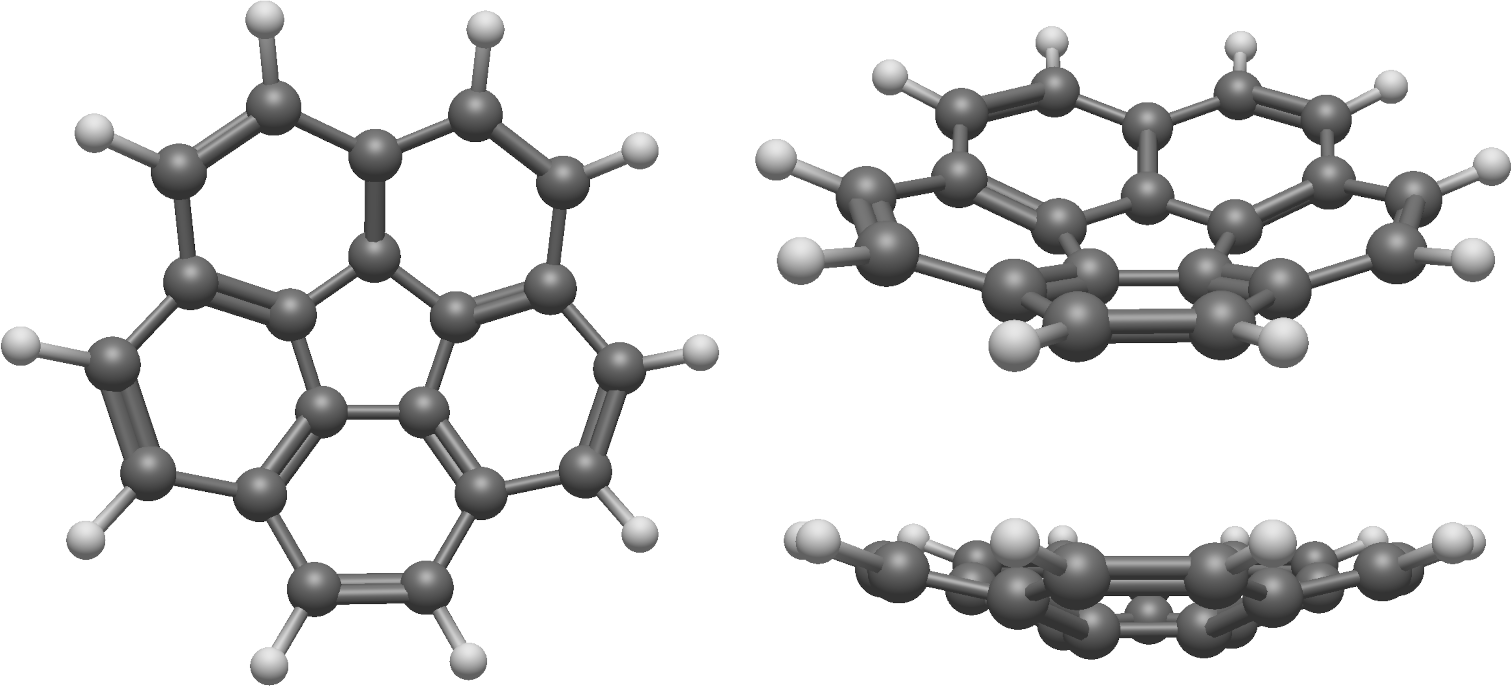
\includegraphics[width=\linewidth]{figures/corannulene.png}
            \caption{Structure of corannulene (\ch{C20H10}), a molecule with $C_{5v}$ symmetry in its ground state, shown from three different perspectives. Note that the carbon atoms are not coplanar in the ground state.}
            \label{fig:corannulene}
        \end{figure}
    \end{frame}

    \begin{frame}{Molecules with fivefold symmetry}
        Corannulene undergoes a bowl-to-bowl inversion process, where it passes through a high energy planar transition state. \cite{mattarella} Its transition state has $D_{5h}$ symmetry, which occurs precisely when it is exactly between the two bowl configurations. This is an interesting example of a phenomenon where molecular motion may momentarily change the point group to which a molecule belongs.

        \begin{figure}[htbp]
            \centering
            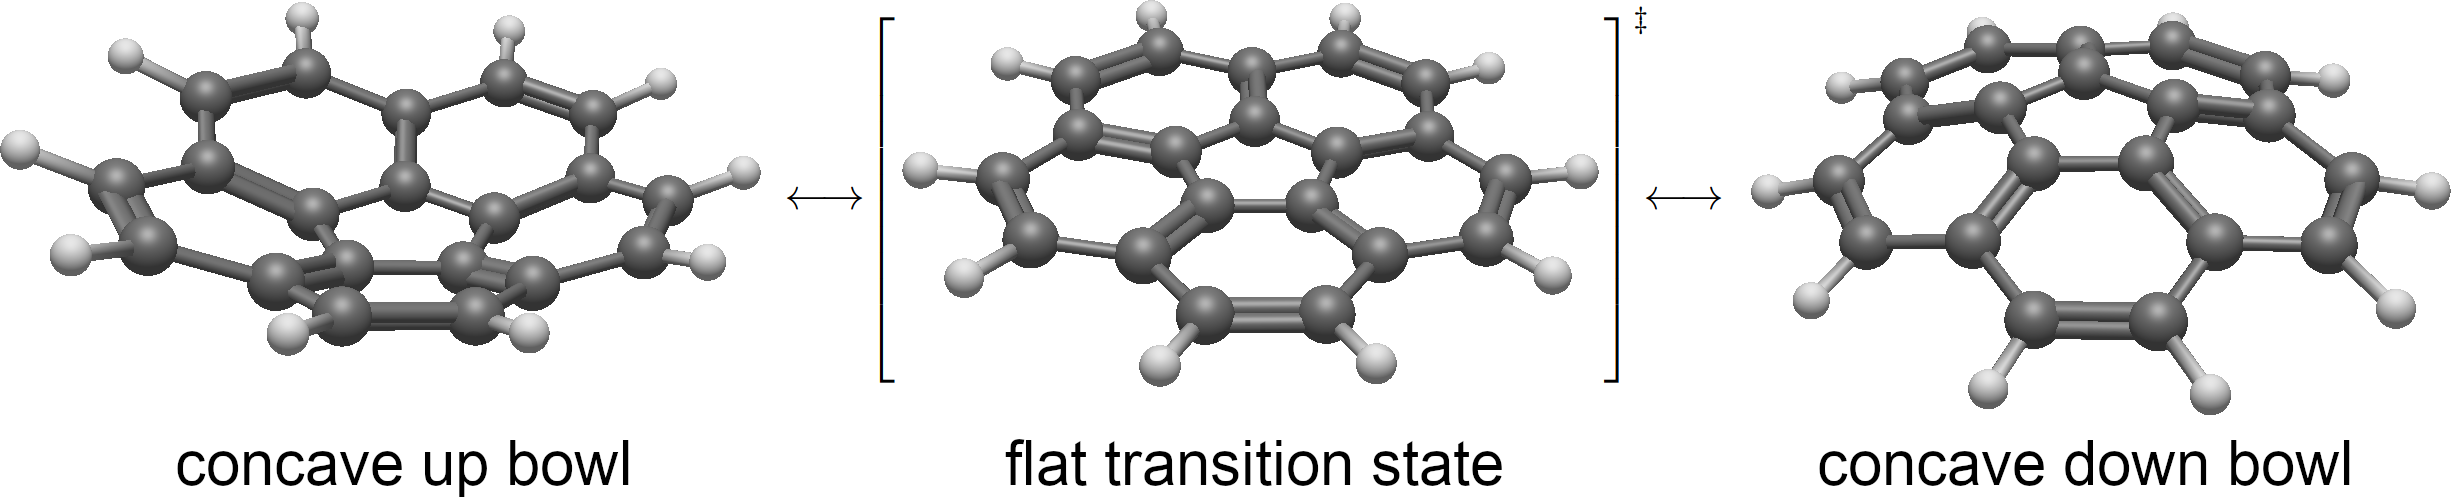
\includegraphics[width=\linewidth]{figures/corannulenebowltobowl.png}
            \caption{Bowl-to-bowl inversion of corannulene, showing the two ground-state bowl configurations with $C_{5v}$ symmetry and the flat transition state (denoted $\ddagger$) with $D_{5h}$ symmetry. \cite{sripaturad}}
            \label{fig:corannulenebowltobowl}
        \end{figure}
    \end{frame}

    \begin{frame}{Molecules with fivefold symmetry}
        Ionizing corannulene also changes the point group to which it belongs. The neutral state of corannulene has a doubly degenerate HOMO and LUMO. Adding an electron to form a negative ion (anion) causes a partial filling of a doubly degenerate LUMO, and removing an electron to form a positive ion (cation) causes a partial filling of a doubly degenerate HOMO. Both of these situations result in a Jahn-Teller effect, where a molecule will undergo a geometric distortion to eliminate degeneracy, thereby reducing symmetry, as seen on the next slide. For that reason, both cationic and anionic forms of corannulene belong to the point group $C_s$, which lacks rotational symmetry and only contains a single $\sigma_h$ mirror plane. \cite{tampieri}
    \end{frame}

    \begin{frame}{Molecules with fivefold symmetry}
        \begin{figure}[htbp]
            \centering
            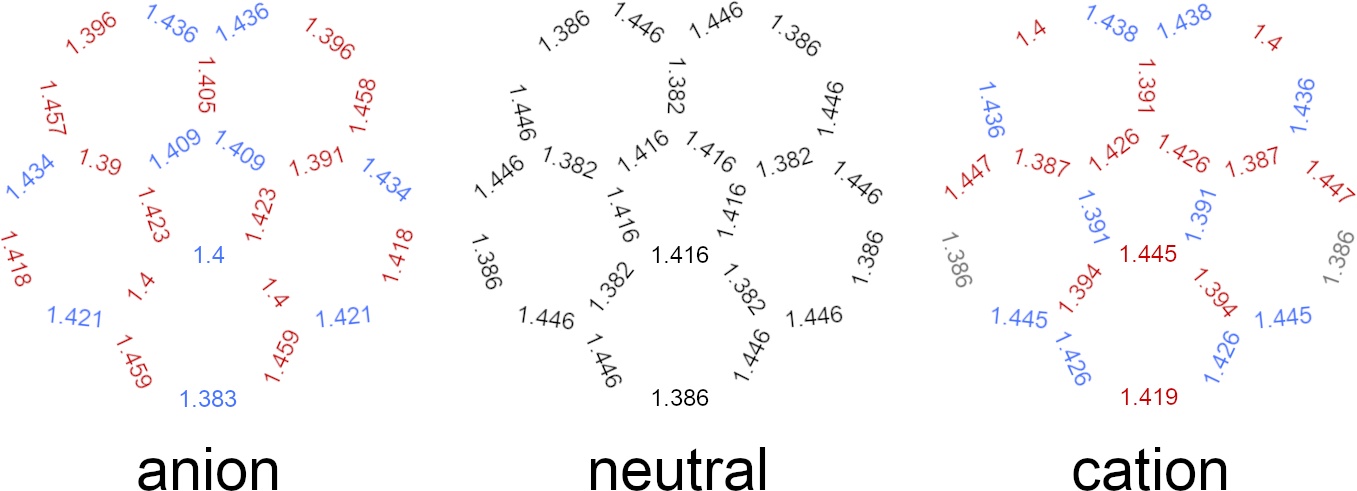
\includegraphics[width=\linewidth]{figures/jahnteller.png}
            \caption{Bond lengths of corannulene, in angstroms (\AA), in the anion form (left), neutral form (center), and cation form (right), illustrating the Jahn-Teller effect. Calculated by Tampieri et al. using Density Functional Theory. Note that the distorted bond lengths in the anion and cation forms reduce the symmetry to the point group $C_s$, as compared to $C_{5v}$ for the neutral form. Colors indicate a change in bond length as compared to the neutral form (red: longer, blue: shorter, gray: no change at three decimal places). \cite{tampieri}}
            \label{fig:jahnteller}
        \end{figure}
    \end{frame}

    \begin{frame}{Molecules with fivefold symmetry}
        Another molecule with fivefold symmetry is ferrocene (\ch{Fe(C5H5)2}), seen in the next slide. Ferrocene consists of two five-carbon rings that ``sandwich'' an iron atom. In the staggered conformation, the rings are flipped relative to each other, and the molecule belongs to the point group $D_{5d}$. In the eclipsed conformation, the two rings are aligned in the same way, and the molecule belongs to the point group $D_{5h}$. \cite{mohammadi} Along the rotational pathway between the staggered and eclipsed conformations, one may also consider an intermediate twisted configuration that belongs to the point group $D_5$, which has no mirror planes. This is another example where molecular motion can change the point group of a molecule.
    \end{frame}

    \begin{frame}{Molecules with fivefold symmetry}
        \begin{figure}[htbp]
            \centering
            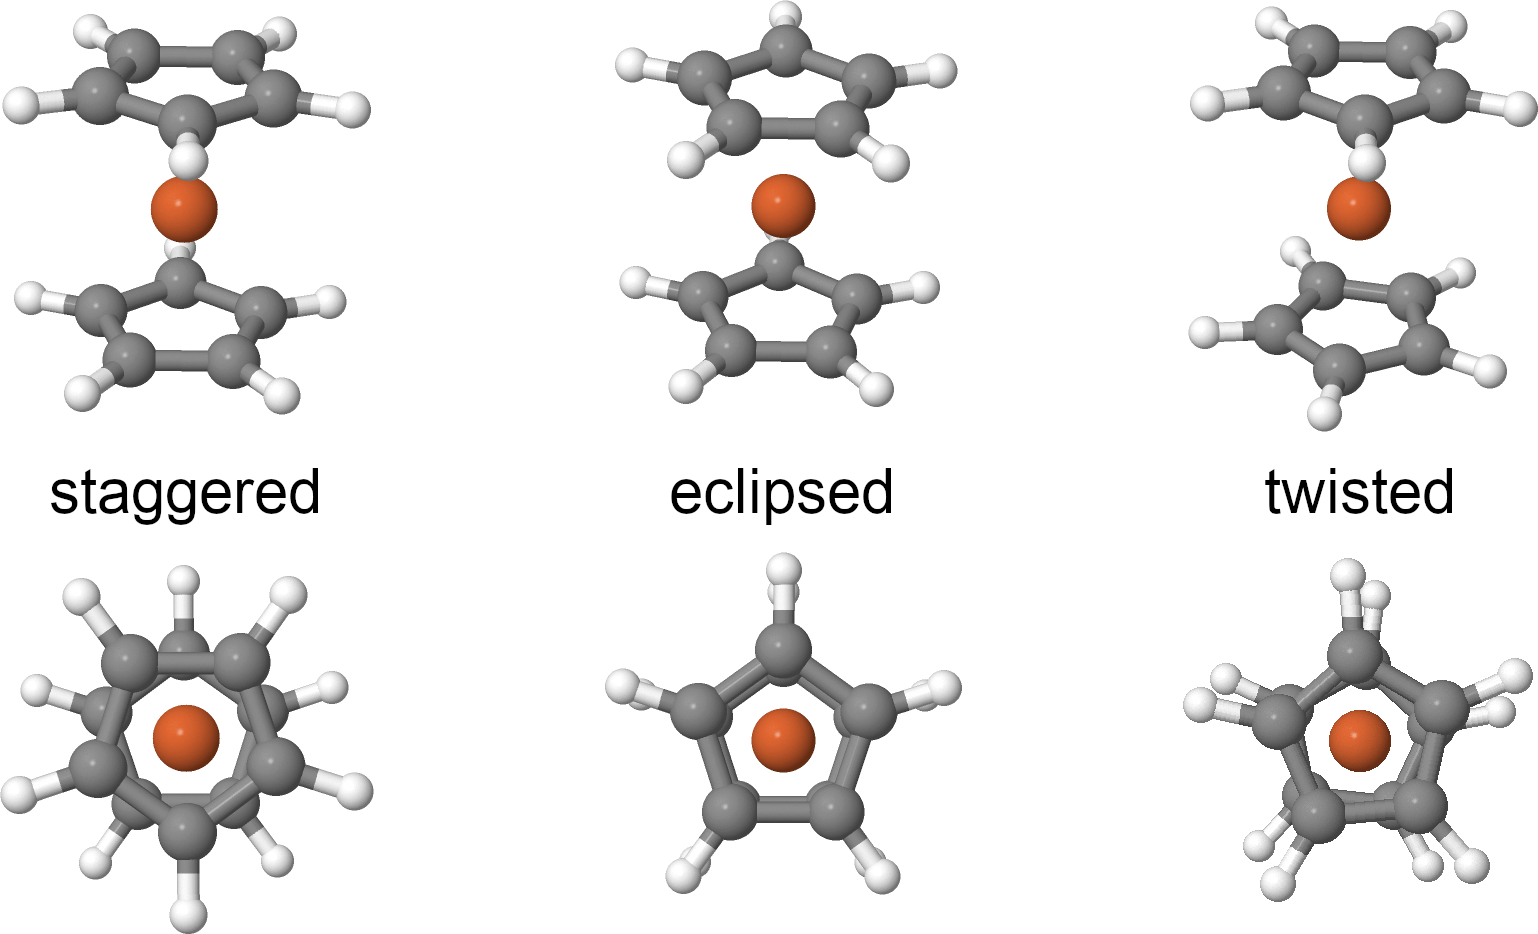
\includegraphics[width=0.75\linewidth]{figures/ferrocene.png}
            \caption{Structure of ferrocene (\ch{Fe(C5H5)2}), a molecule with $D_{5d}$ symmetry in the staggered conformation (left), $D_{5h}$ symmetry in the eclipsed conformation (center), and $D_5$ symmetry in the twisted conformation (right). Each conformer is shown from two perspectives.}
            \label{fig:ferrocene}
        \end{figure}
    \end{frame}

    \begin{frame}{Molecules belonging to abelian point groups}
        We cannot say that \emph{every} point group with fivefold symmetry has character values in $\mathbb{Q}(\sqrt{5})$. The point group $C_5$ is a counterexample. Here, $C_5$ is not referring to a fivefold rotational symmetry operation, but an entire point group, which contains no mirror planes, and no $C_2$ axes perpendicular to the principal $C_5$ axis. The point group $C_5$ is abelian, and it is a cyclic group of order $5$.
        \vs

        \onslide<2->
        {
            Hence, all of its irreps are 1D, so the characters lie in $\mathbb{Q}(\zeta_5)$, not $\mathbb{Q}(\sqrt{5})$. Thus, the appearance of characters in $\mathbb{Q}(\sqrt{5})$ is a feature of point groups with suitable 2D irreps, such as $C_{5v}$, $D_{5d}$, $D_{5h}$, and $D_5$, but not of every point group with fivefold symmetry.
        }
    \end{frame}

    \begin{frame}{Molecules belonging to abelian point groups}
        Molecules belonging to the point group $C_5$ are rare. One fascinating molecule belonging to the point group $C_5$ is 1,3,5,7,9-penta(ferrocenyl)corannulene (\ch{C20H5(C5H5FeC5H4)5}). This molecule consists of a corannulene structure to which five ferrocenyl functional groups are bonded. This molecule provides a concrete realization of the point group $C_5$, illustrating a case where the characters lie in the cyclotomic field $\mathbb{Q}(\zeta_5)$ rather than $\mathbb{Q}(\sqrt{5})$. A 3D rendering of this molecule is shown on the next slide. \cite{miessler2014,topolinski}
    \end{frame}

    \begin{frame}{Molecules belonging to abelian point groups}
        \begin{figure}[htbp]
            \centering
            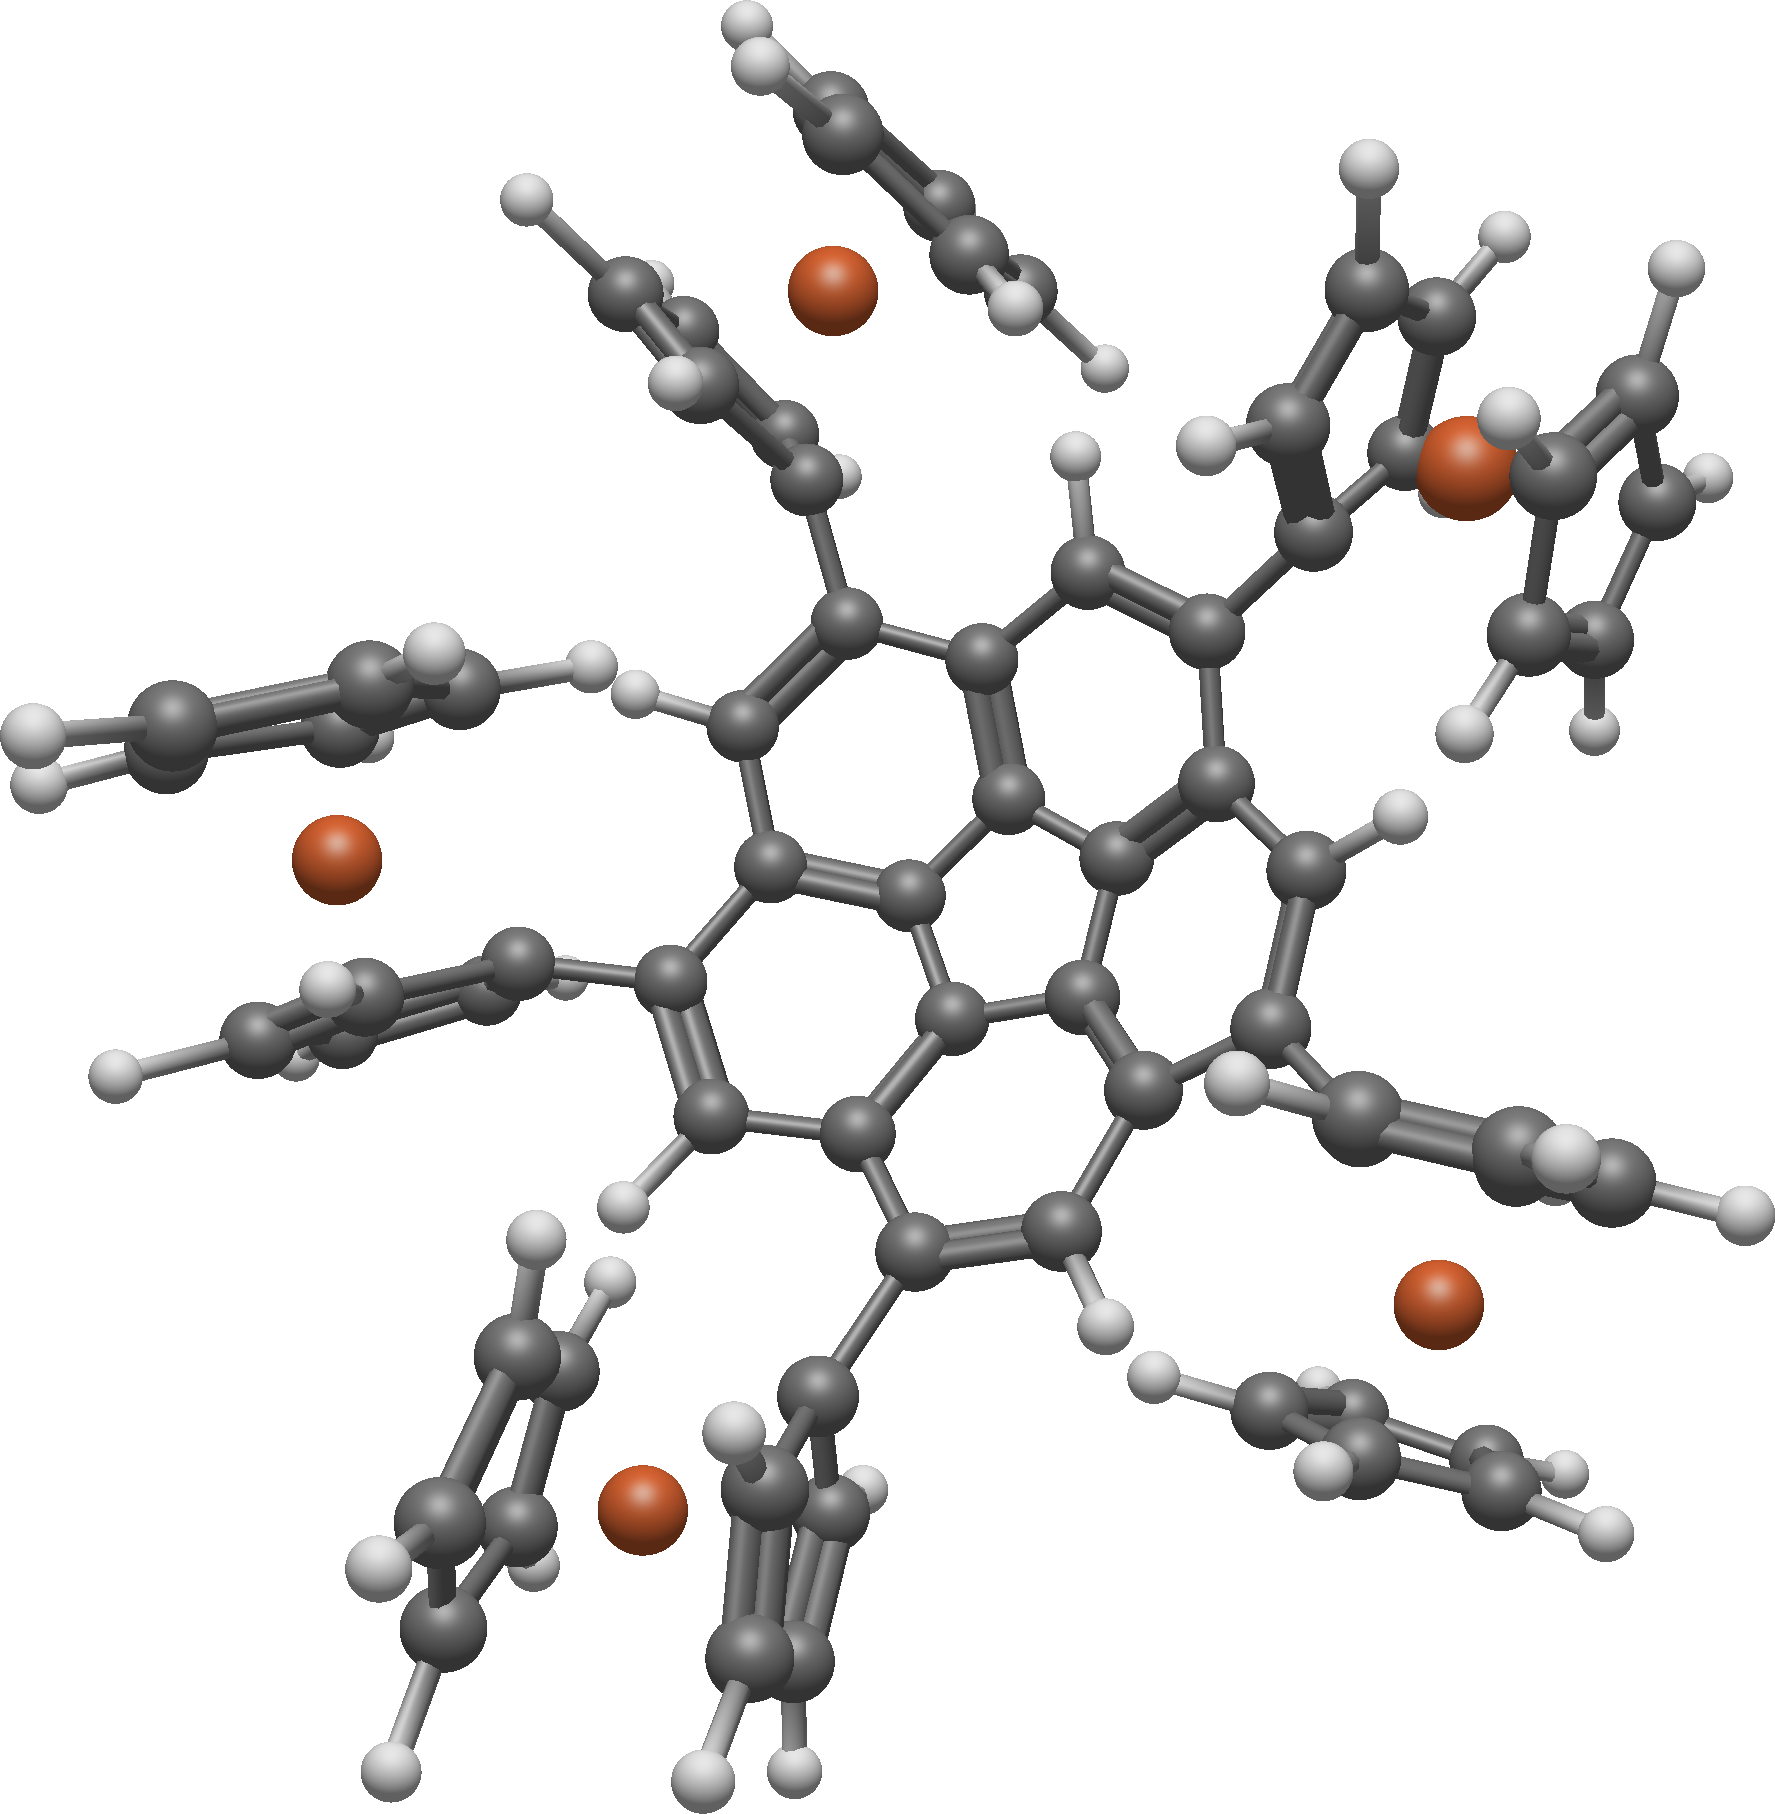
\includegraphics[width=0.45\linewidth]{figures/fercor.png}
            \caption{Structure of 1,3,5,7,9-penta(ferrocenyl)corannulene (\ch{C20H5(C5H5FeC5H4)5}), a molecule with $C_5$ symmetry. The ``concave up'' side of the corannulene bowl structure is facing the reader. Original artwork based on a skeletal structure provided by Topolinski et al. \cite{topolinski}}
        \end{figure}
    \end{frame}

    \begin{frame}{Molecules belonging to abelian point groups}
        Likewise, not every point group with threefold symmetry has character values in $\mathbb{Z}$. The point group $C_3$ is a counterexample. This is an abelian point group, and it contains no mirror planes and no $C_2$ axes perpendicular to the principal $C_3$ axis. Its irreps are 1D, so the characters lie in $\mathbb{Q}(\zeta_3)$, not $\mathbb{Z}$.
        \vs

        \onslide<2->
        {
            As with the point group $C_5$, molecules belonging to the point group $C_3$ are uncommon. One molecule belonging to the point group $C_3$ is triphenylphosphine (\ch{P(C6H5)3}). This molecule has trigonal pyramidal geometry, similar to ammonia. The skeletal structure of this molecule is shown on the next slide. \cite{miessler2014}
        }
    \end{frame}

    \begin{frame}{Molecules belonging to abelian point groups}
        \begin{figure}[htbp]
            \centering
            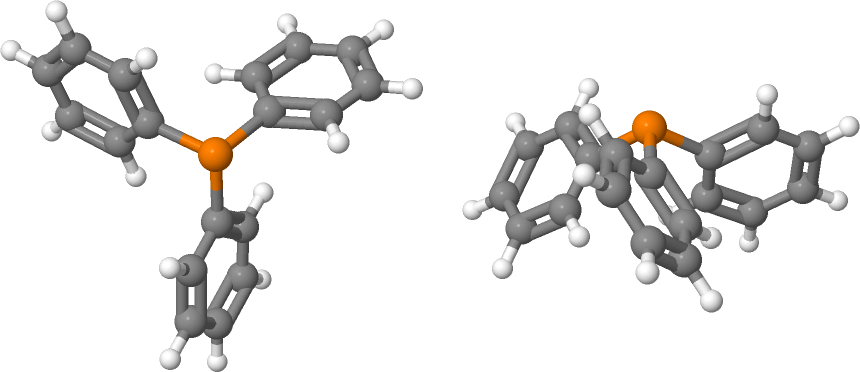
\includegraphics[width=\linewidth]{figures/pph3.png}
            \caption{Structure of triphenylphosphine (\ch{P(C6H5)3}), a molecule with $C_3$ symmetry, shown from two perspectives.}
            \label{fig:pph3}
        \end{figure}
    \end{frame}

    \begin{frame}{Future directions}
        \begin{itemize}
            \item Expand the scope into other point groups, such as those of high symmetry ($T_d$, $O_h$, $I_h$), those with other orders ($C_{4v}$, $D_{6h}$, $D_{8h}$), and $D_n$ or $S_{2n}$, to determine how the associated character fields vary systematically with the structure of the point group.
            \item Analyze linear point groups such as $C_{\infty v}$ and $D_{\infty h}$. Here, the finite group framework is replaced by continuous symmetry groups related to the Lie groups $SO(2)$ and $O(2)$. This suggests a broader perspective in which molecular symmetry connects naturally to the representation of Lie groups and Fourier analysis.
            \item The focus of this work on geometric (Cartesian) representations, along with permutation-type representations arising from atomic positions (not presented to save time). A natural extension would be to investigate whether the same cyclotomic and Galois-theoreic structure appears in other representations commonly used in chemistry, such as vibrational representations or those arising in molecular orbital theory.
        \end{itemize}
    \end{frame}

    \begin{frame}{Questions?}
    
    \end{frame}

    \begin{frame}{Acknowledgments}
        I would like to express my most sincere gratitude to my advisor, Dr.\ Lilit Martirosyan, for her guidance, encouragement, and insightful feedback throughout this project.
        \vs

        I am also grateful to Dr.\ Sean English for his engaging teaching and for continually challenging me to think more deeply about mathematics, and to Dr.\ Russell Herman for his instruction and influence on my mathematical curiosity and development.
        \vs

        I would like to thank Dr.\ Nicholas Chiappini for carefully reviewing the chemistry in this paper, as well as Dr.\ Erik Slivken for this thoughtful input. I am also thankful to Dr.\ Dijana Jakelic for the opportunity to present my work and offer constructive feedback.
    \end{frame}

    \begin{frame}{Acknowledgments}
        I would also like to acknowledge Dr.\ Thomas Coombs, Dr.\ Bart Jones, and Dr.\ Robert Hancock, whose teaching helped me develop my knowledge and interest of chemistry.
        \vs

        I am grateful to my classmates for their encouragement and support throughout this process. Finally, I would like to thank my wife, Samantha, and my pets for their unwavering love, support, and patience.
    \end{frame}

    \begin{frame}[allowframebreaks]{References}
        \printbibliography[heading=bibnumbered]
    \end{frame}
\end{document}